\documentclass{article}
\usepackage[utf8]{inputenc}
\usepackage{amsmath,amsfonts,amssymb}
\usepackage{xcolor}
\usepackage{cleveref}
\usepackage{graphicx}
\usepackage{physics}
\usepackage{tikz}
\usepackage{lmodern} 
\usepackage{csquotes}
\DeclareRobustCommand\full  {\tikz[baseline=-0.6ex]\draw[thick] (0,0)--(0.5,0);}
\DeclareRobustCommand\Rfull  {\tikz[baseline=-0.6ex]\draw[red,thick] (0,0)--(0.5,0);}
\DeclareRobustCommand\dotted{\tikz[baseline=-0.6ex]\draw[thick,dotted] (0,0)--(0.54,0);}
\DeclareRobustCommand\dashed{\tikz[baseline=-0.6ex]\draw[thick,dashed] (0,0)--(0.54,0);}
\usepackage{adjustbox}
\usepackage{multirow}
\usepackage{subcaption}
\usepackage{MnSymbol}
\usetikzlibrary{positioning,3d}
\usetikzlibrary{graphs,automata}
\usepackage{biblatex}
\usepackage{float}
\usepackage{pgfplots}
\usetikzlibrary{backgrounds}
\pgfplotsset{compat=1.15
 ,colormap={parula}{
rgb255=(53,42,135)
rgb255=(15,92,221)
rgb255=(18,125,216)
rgb255=(7,156,207)
rgb255=(21,177,180)
rgb255=(89,189,140)
rgb255=(165,190,107)
rgb255=(225,185,82)
rgb255=(252,206,46)
rgb255=(249,251,14)
        }}



\usetikzlibrary{patterns}
\usepackage[english]{babel}
\addbibresource{bibliography.bib}
\addbibresource{roughness.bib}

\crefformat{section}{\S#2#1#3} % see manual of cleveref,
\crefformat{subsection}{\S#2#1#3}
\crefformat{subsubsection}{\S#2#1#3}

\title{DNS-based characterization of pseudo-random roughness in minimal channels}
\author{Jiasheng Yang }
\date{July 2020}

\begin{document}

\maketitle
\begin{abstract}
    In present work, we discuss an efficient technical routine for a comprehensive study of roughness.
    Direct numerical simulation (DNS) is used to study flow over a number of artificial irregular rough surfaces in periodic plane channels.
    The idea of conducting DNS on irregular roughness in minimal channels is applied and examined in this work.
    To this end, DNS results of flow in channels with smaller spanwise sizes are compared to those in large channels with $Re_\tau$ from 250 up to 1000 to cover transitionally rough and fully rough regimes.
    Generation of the irregular rough surface is based on a mathematical random algorithm in which the height power spectrum of the roughness elements (PS) along with its height probability distribution (HPD) can be prescribed.
    Different types of rough surfaces characterized in terms of HPD and PS are generated and evaluated.
    The roughness generation approach allows generation of roughness samples that may be considered as surrogate of realistic roughness and can replace the costly process of scanning industrial surfaces.
    multiple existing roughness correlations are assessed in present work, suggestion of including both HPD information and PS information in correlation is given. 
    %A Neural Network (NN) as well as a Gaussian Progress Regression (GPR) machine learning model are trained for the prediction of roughness function $\Delta U^ +$basing on the simulation results at $Re_\tau\approx500$. It is proven that with HPD and PS for a roughness informed, a predictive tool of roughness function $\Delta U^+$ can be developed, maximum prediction error of $3\%$ is achieved.
\end{abstract}
\section{Introduction}
Turbulent flows bounded by rough walls are abundant in nature (e.g. fluvial flows \cite{mazzuoli17} and wind flow over vegetation~\cite{SHAW198251} or urban canopies~\cite{coceal04,yang16}) and industrial applications (e.g. degraded gas turbine blades \cite{bons01}, bio-fouled ship hulls \cite{hutchins16}, iced surfaces in aero-engines~\cite{Juan2019} and deposited surfaces inside combustion chambers~\cite{FOROOGHI201883}). Systematic study of roughness effects on skin friction dates back to the pioneering works of Nikuradse~\cite{Nikuradse1933} and Schlichting~\cite{schlichting1936experimentelle}. For industrial applications Moody diagram~\cite{Moody1944} has been considered the standard method to calculate the skin friction of a rough surface. It must be reminded that Moody diagram relates the friction factor to the equivalent sand-grain roughness height $k_s$, a quantity that is not known \textit{a priori} for any arbitrary rough surface. Hence, for a new roughness topography, this quantity needs to be determined using a laboratory or high fidelity numerical experiment or based on a roughness correlation derived from such experiments.\\

The problem of predicting the roughness-induced friction drag merely based on the knowledge of the roughness topography has received extensive attention in the past, and a variety of roughness correlations have been developed in different industrial contexts \cite{Sigal,waigh98,Rij,macdonald00,BONSRA,flack2010,chan2015,FOROOGHI201883,thakkar17,Flack2020}. In these roughness correlations, the topography of the rough surface is often represented by statistical measures of the roughness height map $k(x,z)$, $k$ being the surface height as a function of horizontal coordinates $x$ and $z$. Some widely discussed statistical measures in this context are skewness $Sk=\frac{1}{k_{rms}^3}\int_S(k-k_{md})^3dS$ \cite{flack2010,10.1115/1.4037280}, effective slope $ES=\frac{1}{S}\int_S|\frac{\partial k}{\partial x}|dS$~\cite{napoli_armenio_de_marchis_2008,chan2015}, density parameter $\Lambda_s=({S}/{S_f})({S_f}/{S_s})^{-1.6}$~\cite{Sigal,Rij}, and correlation length $L_x^{corr}$ (the streamwise distance by which the autocorrelation function of $k$ falls below a certain threshold) \cite{Thakkar2017}. Here $k_{rms}=(\frac{1}{S}\int_Sk^2dS)^{1/2}$ and $k_{md}$, $S$, $S_s$, and $S_f$ denote the mean roughness height (melt-down height), total wall-parallel projected area, total windward wetted area, and total frontal projected area of the roughness.
Furthermore, $k_a=\frac{1}{S}\int_S|k-k_{md}|dxdz$ is the averaged absolute height deviation from melt-down height~\cite{chan_macdonald_chung_hutchins_ooi_2015}.\\

Despite extensive work in the past, a universal correlation with the ability to accurately predict the drag of a generic rough surface remains elusive \cite{flack18}. Arguably, development of such a correlation requires a large amount of data from realistic roughness samples. However, generation of such a database has been hindered mainly due to two factors; first, the formidable cost associated with many (numerical) experiments. Second, the relative scarceness of realistic roughness maps and lack of ability to systematically vary their properties. The present report outlines an attempt by the authors to introduce a framework that resolves both issues.\\

As a matter of fact, a considerable portion of available data in the literature deal with regular roughness - often generated by distribution of similar geometric elements. Examples of studied geometries include cubes~\cite{Orlandi06,leonardi_castro_2010}, spheres~\cite{mazzuoli17}, pyramids~\cite{Schultz2010}, LEGO bricks~\cite{placidi_ganapathisubramani_2015}, ellipsoidal egg-carton shape~\cite{Bhaganagar2008}, and sinusoidal roughness~\cite{chan_macdonald_chung_hutchins_ooi_2015,chan_macdonald_chung_hutchins_ooi_2018}. In comparison, investigations based on realistic rough surfaces are less frequent and include a much lower number of cases. Notably, Thakkar et al.~\cite{thakkar17} utilized direct numerical simulation (DNS) to study the effect of roughness topography on flow statistics for 17 industrially relevant irregular surfaces and proposed roughness correlations for transitionally rough regime. Other examples of realistic roughness studies in the framework of wall-bounded turbulence include~\cite{cardillo_chen_araya_newman_jansen_castillo_2013,yuan14,BUSSE2015129,busse_thakkar_sandham_2017,FOROOGHI201883,Yuan2018}\\

In recent years, mathematically generated irregular roughness has received an increased attention as a means to systematically approach a universal roughness correlation. One of the earliest attempts of this kind was made by Scotti~\cite{scotti2006} who proposed a method to produce virtual sand roughness by random distribution of ellipsoids. Others adopted randomized roughness generation concepts based on discrete elements~\cite{10.1115/1.4037280,Forooghiheattransfer,kuwata_kawaguchi_2019}, ripples~\cite{chau2012} or superposition of sinusoids~\cite{napoli_armenio_de_marchis_2008,demarchis20} to generate irregular roughness. In an attempt to study turbulence over surfaces that closely resemble realistic roughness, Jelly and Busse~\cite{jelly19} generated height maps, $k(x,z)$, using weighted linear combinations of Gaussian-distributed random numbers.
In their large eddy simulation (LES) study focused on realistic complex terrain, Anderson and Meneavue~\cite{anderson_meneveau_2011} used random Fourier modes to create surfaces with power-law power spectra ($E(q)\propto q^p$ - where $q$ is the wave number and $p$ is a constant).
Barros et al.~\cite{BARROS20181} employed a modified version of this roughness generation method to study the effect of spectral slope $p$ on the friction drag using wind tunnel boundary layer experiments. It must be noted that while the power spectrum (PS) of roughness height determines the distribution of roughness wavelengths (horizontal scales), it does not control the probability distribution function (PDF) of roughness height, which is another important factor. In this respect, while the majority of the above cited works deal with Gaussian PDFs, naturally occurring roughness can be highly non-Gaussian \cite{bons01,thakkar17}.
Indeed many previous studies highlighted significant impact of of departure from Gaussian distribution -- mainly measured by skewness -- on the mean flow and turbulent statistics \cite{flack2010,jelly_busse_2018,FOROOGHI201883,kuwata_kawaguchi_2019}.
Motivated by that, recently Flack and co-workers (Flack et al.~\cite{Flack2020}) generated non-Gaussian rough surfaces using the Pearson system random numbers, in which the skewness and kurtosis of the PDF can be prescribed. These mathematically generated surfaces were then tested in a water channel facility to determine the relation between $k_s$ and skewness in realistic roughness. In the present paper we adopt an alternative roughness generation method~\cite{PEREZRAFOLS2019591}, which provides the flexibility to prescribe any desired combination of PDF and PS. The algorithm offers more robustness and freedom (prescribing the PDF  rather than a few moments) compared to the algorithms based on translations of Pearson's or Johnson's types~\cite{PEREZRAFOLS2019591} and can be utilized for generation of roughness samples that serve as surrogates of realistic roughness in friction drag studies. We refer to the roughness samples generated by this method as `pseudo-random' roughness hereafter.\\
%%%%%%%%%%%%%%%%%%%%%%%%%%%%%%%%%%%%%%%%%%%%%%%%%%%%%%%%%55
%Summarize previous works on minimal channel for roughness in one paragraph....\\

As mentioned above, both experiments and numerical simulations are employed in the past to study turbulent flows over rough walls. Multiple experiment and simulation campaigns have been conducted in roughened pipes ~\cite{Nikuradse1933,langelandsvik_kunkel_smits_2008,chan_macdonald_chung_hutchins_ooi_2015}, developing boundary layers~\cite{flack07,cardillo_chen_araya_newman_jansen_castillo_2013,BarrosBL2019}, channels~\cite{flack16,napoli_armenio_de_marchis_2008,Bhaganagar2008,Orlandi06} and open channels~\cite{chan-braun_garcía-villalba_uhlmann_2011,10.1115/1.4037280}.
In recent years, DNS has been the pacing approach in studying the effect of roughness topography on friction drag. Standard DNS, however, involves resolving the entire spectrum of turbulent length scales ranging from the large geometrical scales to the small viscous scale, which is computationally costly. For wall-bounded turbulence simulations the cost of DNS scales with $Re_\tau^ 3$~\cite{pope_2000}, which means that covering a wide roughness topography parameter space by DNS is prohibitively expensive even at moderate Reynolds numbers.   
%With the aim of simulating roughness in fully rough regime, computational cost can be excessively raised, which holds researchers back from conducting a massive number of DNS simulations.
%However it is reported by Townsend~\cite{Townsend} that roughness has a major effect in the vicinity of wall labeled as 'roughness sub-layer'.
%The flow outside the roughness sub-layer remains unaffected when scaling in wall unit. 
%From this point of view, accurate simulation of near wall flow is of core importance.
To tackle this problem, Chung et al.~\cite{chung_chan_macdonald_hutchins_ooi_2015} employed the idea of DNS in minimal span channels~\cite{jimenez_moin_1991} for prediction of roughness-induced drag over a regular sinusoidal roughness in a channel. The central idea followed by these authors is that the amount of downward shift in the inner-scaled velocity profile $\Delta U^+$ is the determining factor in prediction of drag, and thanks to outer layer similarity of wall bounded turbulence~\cite{Townsend}, this quantity can be accurately predicted as long as an adequately large range of near-wall structures are accommodated in the simulation domain. Despite exclusion of larger structures, which leads for the solution to be nonphysical in the outer layer, these authors could predict $\Delta U^+$ accurately. The same group of authors further developed the idea for channels with minimal streamwise extent~\cite{MacDonald_2016} and also for passive scalar calculations ~\cite{macdonald_chung_hutchins_chan_ooi_garcía-mayoral_2017}. These efforts established to the following criteria for the size of a minimal channel basing on the simulations with minimal channels on 3D sinusoidal roughness.
\begin{equation}
L_z^+\geq \text{max}(100,\frac{\Tilde{k}^+}{0.4},\lambda_{sin,z}^+)
\label{MINI2}
\end{equation}
\begin{equation}
L_x^+\geq \text{max}(1000,3L_z^+,\lambda_{sin,x}^+)
\label{MINI1}
\end{equation}
where $L_z$ and $L_x$ are the spanwise and streamwise extent of the minimal channel, respectively, $\lambda_{sin}$ is the sinusoid wavelength of roughness, $\Tilde{k}$ is the characteristic roughness height (here sinusoid amplitude) and the plus superscript indicates viscous scaling. % $U_\tau=\sqrt{\tau_0/\rho}$ is friction velocity, $\tau_0$ is the wall drag force per plan area. 
MacDonald et al.~\cite{macdonald_hutchins_chung_2019} also showed that the calculated flow field can be considered physical up until a critical height $y_c\approx0.4L_z$.\\

While the aforementioned efforts showed the potential of using minimal channels for study of roughness-induced drag an extension of this concept to irregular roughness is yet to made. One must specifically note that, the roughness originally studied by Chung and co-workers ~\cite{chung_chan_macdonald_hutchins_ooi_2015,macdonald_chung_hutchins_chan_ooi_garcía-mayoral_2017,macdonald_hutchins_chung_2019} composes of repetitive sinusoidal patterns meaning that the roughness geometry of a minimal channel is an exact subset of the original surface. For realistic roughness, it is important to understand if the same concept can be applied when the minimal and the original roughness samples are merely statistically similar. Recently, Portela and Sandham \cite{alves20} attempted to predict flow over a realistic roughness combining minimal channels with a novel hybrid DNS/URANS model. While their hybrid model generated similar results to pure DNS in channel with the same size, their predicted $k_s$ in minimal channels did not necessary match those in the larger ones. This further highlights the need for careful investigation of minimal channel concept for realistic roughness. \\

%%%%%%%%%%%%%%%%%%%%%%%%%
In the present work, we use the flexibility provided by the pseudo-random roughness generation algorithm to systemically study the application of minimal channel concept for irregular roughness. Unlike the previous works, in which minimal geometries are geometrically similar subsets of the original roughness geometry, we study 'statistically' similar surfaces. In doing so, we aim to address two research questions; on one side, we propose generalized rules for the size requirements of the minimal channel for any arbitrary rough surface. On the other side, we shed light on the statistical properties that can uniquely describe hydrodynamic properties of roughness. To ensure the generalizability of our answers the problem is studied for a wide range of roughness types and also for both transitionally and fully rough regimes.




%Flows bounded by rough walls are abundant in natural and industrial applications e.g. flow over canopies~\cite{SHAW198251}, urban wind~\cite{Grimmond}, combustion chamber deposits~\cite{FOROOGHI201883}, ice accretion on aero-engine intake~\cite{Juan2019}, etc..
%The presence of roughness intensifies the turbulence in the vicinity of rough wall thus increase the skin friction as well as heat transfer ability~\cite{Forooghiheattransfer}, which translates to an altered energy conversion efficiency.
%It is observed that a rough surface can increase both skin friction and heat exchange to different extend.
%Bons et al.~\cite{BONSRA} introduced Reynolds analogy factor $RA=\frac{2St}{C_f}$ to quantify the alteration of heat and momentum exchange by rough wall, where $St$ is Stanton number while $C_f$ is the friction factor.
%Therefore the study of roughness can be the relevant topic to the area of environmental protection.
%It is well established that in the vicinity of roughness downward velocity profile shift or retardation in the mean flow relative to smooth cases can be observed~\cite{BoundarylayerT}.
%This downward velocity shift is denoted as (Hama) roughness function $\Delta U$~\cite{hama1954}, which is often used to quantify the drag force exerted by roughness.
%The log law of rough pipe writes~\cite{Nikuradse1933}
%\begin{equation}
%    U^+=\frac{1}{\kappa}ln(y^+)+B-\Delta U^+
%\end{equation}
%Where $\kappa\approx0.4$ is the von Karman constant, B is the log-law intercept for the smooth wall, superscript + indicates wall unit scaling.
%From previous work by Nikuradse~\cite{Nikuradse1933}, three flow regimes over roughness are observed with the increasing Reynolds number, namely 'hydraulically smooth' regime, 'transitionally rough' regime and 'fully rough' regime.
%Particularly in fully rough regime friction coefficient $C_f$ becomes constant, resistance is predominantly determined by the pressure drag induced by roughness protuberance~\cite{jouybari2020datadriven}.
%Thus the friction is solely a function of roughness size.
%The roughness function writes~\cite{ligrani_moffat_1986}
%\begin{equation}
%    \Delta U^+ =B-8.48+\frac{1}{\kappa}ln(k_s^+)
%    \label{asysptot}
%\end{equation}
%where $k_s$ is the sand grain size taken from Nikuradse's research on rough pipes~\cite{Nikuradse1933}, where roughness are produced by uniform sand grain size $k_s$.
%Moody~\cite{Moody1944} extended the research basing on experiments on industrial pipes with arbitrary roughness, $k_s$ of arbitrary roughness is referred to as equivalent sand-grain size which induces the same skin friction in the fully rough regime as Nikuradse's experiments.
%Therefore $k_s$ is a hydrodynamic property rather than a physical property.
%Once $k_s$ is determined, hydraulic drag can be predicted using Moody's chart~\cite{Moody1944}.\newline 
%As stated, $k_s$ is of significant role in the prediction of skin friction which can only be obtained by well-controlled laboratory experiments or high-fidelity simulations. 
%A priori prediction of $k_s$ basing on its topographical properties is since long demanded. 
%Since decades researchers have been working on establishing the correlation of roughness topographical properties with equivalent sand-grain size $k_s$. 
%For k-type rough surfaces, proportional relationship of effective roughness height $k$ and $k_s$ is reported~\cite{ktype}, therefore $k_s=k_{ref}\cdot k_r$.
%Where $k_{ref}$ is the characteristic height of roughness element, for instance, $k_{ref}$ is taken as the r.m.s. of roughness elevation $k_{rms}=(\frac{1}{S}\int_Sk^2dS)^{1/2}$~\cite{flack2010}~\cite{Flack2020} or averaged peak height of roughness $k_p$~\cite{Rij}~\cite{BONSRA}.
%On the other hand $k_r$ is the reduction coefficient~\cite{FOROOGHI201883}.
%It is believed that a wide range of statistical properties of the rough surface can be involved in determining $k_r$ e.g. skewness $Sk=\frac{1}{k_{rms}^3}\int_S(k-k_{md})^3dS$~\cite{flack2010}~\cite{Flack2020}, effective slope $ES=\frac{1}{S}\int_S|\frac{\partial k}{\partial x}|dS$~\cite{10.1115/1.4037280}~\cite{napoli_armenio_de_marchis_2008}, density factor $\Lambda_s=\frac{S}{S_f}\frac{S_f}{S_s}^{-1.6}$~\cite{Rij}, etc. where $k_{md}$ is the meltdown height of roughness, $S$ is the total wall-parallel projected area, $S_s$ is the total windward wetted surface area, $S_f$ is the total projected frontal roughness area.
%Sigal et al.~\cite{Sigal} proposed the correlation
%\begin{equation}
%    ln(k_r)=a\cdot ln(\Lambda_s)+b
%\end{equation}
%Where $a$ and $b$ are empirical value to fit the experiment data, piece-wise-defined correlation is introduced.
%Flack and Schultz~\cite{flack2010} proposed the correlation for whose $ES$ higher than a certain threshold $ES\geq0.35$
%\begin{equation}
%    k_r=A(1+Sk)^{B}
%\end{equation}
%In their most recent study~\cite{Flack2020} $A$ and $B$ are defined differently corresponding to positive/negative $Sk$.
%Bons et al.~\cite{BONSRA} proposed the correlation involving mean surface angle $\overline{\alpha}=\frac{1}{S}\int_Sarctan(\frac{\partial k}{\partial x})dS$
%\begin{equation}
%    k_r=0.0191\cdot \overline{\alpha}^2+0.0736\cdot\overline{\alpha}
%\end{equation}
%However all correlation at the moment show its shortage in predicting universal roughness.
%It is suggested that more geometrical parameters should be involved in correlation~\cite{jouybari2020datadriven}~\cite{10.1115/1.4037280}. 
%Nevertheless, a great number of roughness data are required. 
%In summary, developing a universal roughness predictive tool poses its difficulty due to:
%\begin{itemize}
%    \item[1] Technical difficulties associated with digitization of rough surfaces.
%    \item[2] Limited number of available scanned surfaces leading to a lower variety of roughness property
%    \item[3] Large computational resources required for DNS 
%\end{itemize}
%In order to minimize the effort of producing rough surface data characterized by desired geometrical property, regular roughness, for example surfaces roughened by riblets~\cite{goldstein_tuan_1998}, spheres~\cite{chan-braun_garcía-villalba_uhlmann_2011}, sinusoidal wave~\cite{chan_macdonald_chung_hutchins_ooi_2015}, etc. are generated both digitally~\cite{10.1115/1.4037280} and concretely~\cite{BARROS20181}\cite{Flack2020}.
%However these regular roughness are not representative to most of the realistic roughness due to the lack of richness of roughness topographical scale~\cite{BUSSE2015129}~\cite{BarrosBL2019}. 
%Forooghi et al.~\cite{10.1115/1.4037280} produced rough surface by arbitrarily placing roughness elements in random sizes with prescribed shape onto smooth surface. 
%They also showed that irregular placement of roughness elements can vary the hydraulic property to a considerable extent. 
%Barros et al.~\cite{BARROS20181} used moving average(MA) method to generate irregular roughness, they systematically investigated effect of power spectrum of rough surfaces while the effect of anisotropy is investigated by Busse et al.~\cite{BUSSE2020} using same generation algorithm. 
%However the roughness height distribution is limited to Gaussian. 
%In the most recent research by Flack et al.~\cite{Flack2020} a number of artificially generated non-Gaussian rough surfaces are investigated experimentally, the crucial roles played by the Skewness $Sk$ of height probability distribution as well as the r.m.s. height $k_{rms}$ in characterizing roughness are reported.\newline
%In present work a mathematical \textit{pseudo-random rough surface} generation algorithm is employed which is proposed by Pérez-Ràfols~\cite{PEREZRAFOLS2019591}.
%Both height distribution of roughness elements as well as the spatial distribution of roughness elements can be manipulated (hence the term 'pseudo-random' rough surface).
%The generation algorithm has the advantage in its low effort in generating rough surface of interest.
%On the other hand, roughness properties can thus be parametrically varied, which is ideal for a systematic study of roughness.\newline
%The algorithm initially takes 2 roughness fields as input, one is generated solely according to the given Height Probability Distribution (HPD) labeled as $Y_h^0$, while the other is generated corresponding to given Power Spectrum (PS) of surface elevation labeled as $Y_{ps}^0$. The generation process done by iteratively adjusting the PS and HPD of the surfaces. Iteration process continues until both fields converged to a stationary state, where normally $Y_h$ and $Y_{ps}$ share identical roughness structures. 
%In order to investigate irregular roughness, both experiments and numerical simulations are carried out by researchers worldwide.
%Multiple experiment and simulation campaigns are conducted in roughened pipes ~\cite{Nikuradse1933}~\cite{langelandsvik_kunkel_smits_2008}, boundary layers~\cite{BarrosBL2019}, channels~\cite{flack16}~\cite{napoli_armenio_de_marchis_2008} and open channels~\cite{stroh_schäfer_frohnapfel_forooghi_2020}~\cite{10.1115/1.4037280}.
%However implementing experiments or simulations are expensive. 
%Especially for numerical simulations, turbulent flow contains a wide spectrum of length scale as well as time scale, which makes numerical simulation resolving all the turbulent structures scaling from biggest geometry scale to viscous length scale resource demanding.
%For wall-bounded turbulence simulations because of the requirement of highly refined time step and spatial grid, the cost of DNS scales as $Re_\tau^ 3$~\cite{pope_2000}. 
%With the aim of simulating roughness in fully rough regime, computational cost can be excessively increased, which holds researchers back from conducting a massive number of DNS simulations.
%However for the determination of equivalent sand roughness $k_s$, the central interest is on predicting the downward shift of mean velocity profile.
%It is reported by Townsend~\cite{Townsend} that roughness has a major effect in the vicinity of wall labeled as 'roughness sub-layer'.
%The flow outside the roughness sub-layer remains unaffected when scaling in wall unit. 
%Therefore, the downward shift of velocity profile tend to be a constant value above a few roughness heights and hold constant in logarithmic layer.
%From this point of view, accurate simulation of near wall flow is of core importance.
%The idea of simulating near wall region with minimal flow unit in a restricted smaller channel is proposed by Jiménez and Moin~\cite{jimenez_moin_1991}.
%Chung and MacDonald with co-workers~\cite{MacDonald_2016} suggested using minimal channel for the prediction of roughness function. 
%The suggestion of minimal channel size are proposed~\cite{chung_chan_macdonald_hutchins_ooi_2015}\cite{macdonald_chung_hutchins_chan_ooi_garcía-mayoral_2017}
%\begin{equation}
%L_x^+\geq max(3L_z^+,1000,\lambda_{r,x}^+)
%\label{MINI1}
%\end{equation}
%\begin{equation}
%L_z^+\geq max(100,\frac{k^+}{0.4},\lambda_{r,z}^+)
%\label{MINI2}
%\end{equation}
%Where $\lambda_r$ is the critical wavelength of roughness, $U_\tau=\sqrt{\tau_0/\rho}$ is friction velocity, $\tau_0$ is the wall drag force per plan area, $L_x$ and $L_z$ are streamwise length and spannwise width of minimal channel respectively.
%It is proven that minimal channel DNS can be used for simulation of regular roughness.
%Due to the narrow shape of the minimal channels, only near-wall flow structures can be captured. 
%Thus the prediction of flow field keeps accurate from wall up until the critical height denoted as $y_c\approx0.4L_z$~\cite{macdonald_hutchins_chung_2019}. 
%In present work, the application of minimal channel is generalized to irregular roughness with friction Reynolds number covering both transitionally rough and fully rough regime $Re_\tau\equiv (H-k_{md})u_\tau/\nu\approx250-1000$.\newline
%With the combination of aforementioned techniques (i.e. \textit{pseudo-random rough surface} generation algorithm and minimal channel DNS) an extensive database of roughness is realizable. 
%With the aim of demonstrating the feasibility, a number of simulations on different synthetic roughness are conducted in both minimal channel and full-span channel sense.
%Three roughness parameters are taken under the scope, namely skewness $Sk$ of HPD, decline slope $p$ of PS and upper cutoff wavelength of roughness $\lambda_0$.
%Detailed study of these parameters is presented in \cref{DNS}.
%The data achieved by present simulations will in addition be used to assess the existing correlations.
%With the convenience brought by the roughness generation algorithm, roughness parameters are now extended to frequency space (i.e. the PS).
%With the final aim, establishing a universal roughness correlation, in sight, a predictive tool is built with variable models i.e. linear regression, neural networks (NN) and Gaussian process regression (GPR). The performance of the models are evaluated by five independently generated irregular roughness.


%In \cref{ML} a predictive tool for roughness function is built, linear regression machine learning operations are performed basing on features extracted from both statistics and frequency space using deep neural networks (DNN) and Gaussian process regression (GPR). Models are compared with which is solely developed basing on statistical properties.\newpage
\section{Numerical methodology}
\label{Numerical}
\subsection{Pseudo-random roughness generation}
As mentioned in the introducion, the roughness generation method proposed by Pérez-Ràfols and Almqvist~\cite{PEREZRAFOLS2019591} is adopted in the present methodology. 
In which both wall-parallel and wall-normal statistical properties of the roughness can be adjusted.
Here wall-parallel properties refer to the PS of the roughness structures and wall-normal properties refer to the PDF of the surface height. %The script is written in MATLAB\textcopyright.\newline
The roughness map is represented by a discrete elevation distribution on a 2-dimensional Cartesian grid. 
The generation algorithm used in the present work takes the target PDF and PS as inputs. 
Transformations between the physical space and spectral space is done by discrete fast Fourier transform.
Initially a roughness map $k_h^0$ is generated which has the prescribed PDF but not necessarily the prescribed PS. This initial map is then corrected in the Fourier space according to the prescribed PS. The output of this stage $k_{ps}^0$, has the desired PS but not necessarily the prescribed PDF. In the present notation, subscripts $h$ and $ps$ indicate that the roughness field has the desired PDF and PS, respectively. This correction process continues for $n$ iterations until both  $k_h^n$ and $k_{ps}^n$ converge to a height map with the target PDF and PS within a predetermined error. 
For more details on the the generation algorithm, the readers are referred to reference ~\cite{PEREZRAFOLS2019591}.\\

\subsection{Direct numerical simulation}
A number of DNS have been carried out in fully developed turbulent parallel channel, in which flow is driven by constant pressure gradient.
Representation of the simulation domain is shown in Fig.~\ref{fig:domain}, where \textit{x,y,z} represents streamwise-, wall-normal- and spanwise directions respectively, velocity components are $u$, $v$, $w$ correspondingly.
The roughness are mounted on both upper wall and lower wall.
Channel half height, which is the distance between the deepest trough in roughness and the centre plane of the channel, is labeled as $H$ and will be used to normalize the geometrical scales.
The incompressible Navier-Stokes equations are solved using the spectral solver SIMSON~\cite{Chevalier}, where wall-parallel directions are discretized by Fourier polynomial, while in wall-normal directions Chebyshev discretization is employed.
Immersed Boundary Method (IBM) based on Goldstein et al.~\cite{goldstein_tuan_1998} is used to model the roughness by introducing external volume force field to the Navier-Stokes equation.
The presently used immersed boundary implementation has been validated and extensively used in previous studies~\cite{stroh_schäfer_frohnapfel_forooghi_2020,FOROOGHI201883}.\\
\begin{figure}[H]
\centering
   % 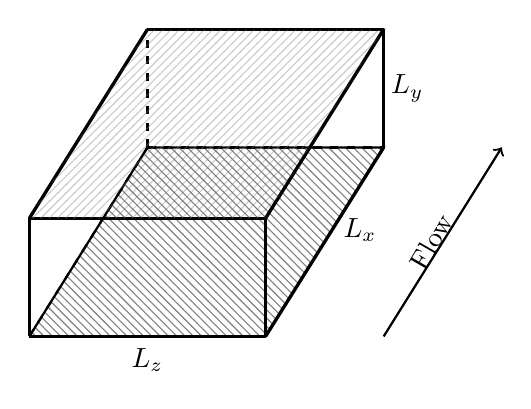
\begin{tikzpicture}[thick,scale=3]
    \coordinate (A1) at (0, 0);
    \coordinate (A2) at (0, 0.5);
    \coordinate (A3) at (1, 0.5);
    \coordinate (A4) at (1, 0);
    \coordinate (B1) at (0.5, 0.8);
    \coordinate (B2) at (0.5, 1.3);
    \coordinate (B3) at (1.5, 1.3);
    \coordinate (B4) at (1.5, 0.8);
    \draw[pattern=north west lines, pattern color=gray] (A1) -- (B1) -- (B4) -- (A4);
    \coordinate (AR1) at (1.5, 0);
    \coordinate (AR2) at (2, 0.8);

    \draw[very thick] (A1) -- (A2);
    \draw[very thick] (A2) -- (A3);
    \draw[very thick] (A3) -- (A4);
    \draw[very thick] (A4) -- (A1);

    \draw[dashed] (A1) -- (B1);
    \draw[dashed] (B1) -- (B2);
    \draw[very thick] (A2) -- (B2);
    \draw[very thick] (B2) -- (B3);
    \draw[very thick] (A3) -- (B3);
    \draw[very thick] (A4) -- (B4);
    \draw[very thick] (B4) -- (B3);
    \draw[dashed] (B1) -- (B4);
    \draw[->] (AR1) -- (AR2);

    %\draw[fill=black!20,opacity=0.5] (A1) -- (A2) -- (A3) -- (A4);
    %\draw[fill=red,opacity=0.6] (A1) -- (A2) -- (B2) -- (B1);
    %\draw[fill=black,opacity=0.6] (B1) -- (B2) -- (B3) -- (B4);
    %\draw[fill=blue,opacity=0.6] (A3) -- (B3) -- (B4) -- (A4);
    \draw[pattern=north east lines, pattern color=gray, opacity=0.4] (A2) -- (B2) -- (B3) -- (A3);
    \node[] at (0.5,-0.10) {$L_z$};
    \node[] at (1.4,0.45) {$L_x$};
    \node[] at (1.6,1.05) {$L_y$};
    \node[rotate=60] at (1.7,0.4) {Flow};
\end{tikzpicture}
   \includegraphics[width=0.8\linewidth]{Figures/Domain.png}
    \caption{Schematic representation of simulation domain, exemplary pseudo-realistic surface is installed}
    \label{fig:domain}
\end{figure}
The Navier-Stokes equation writes
\begin{equation}
    \nabla\cdot \textbf{u}=0
\end{equation}
\begin{equation}
    \frac{\partial \textbf{u}}{\partial t}+\nabla\cdot(\textbf{uu})=\frac{1}{\rho}\nabla p+\nu\nabla^2\textbf{u}+\frac{1}{\rho}P_x\delta_{1i}+\textbf{F}_u
\end{equation}
where \textbf{u} is the velocity vector $\textbf{u}=(u,v,w)^\intercal$, $P_x$ is the mean pressure gradient in flow direction added as a constant source term to the momentum equation to drive the flow in channel. 
Here $p$, $\delta_{1i}$, $\rho$, $\nu$ and $\textbf{F}_u$ are pressure fluctuation, Dirac delta function, density of the flow, kinematic viscosity and external body force term due to IBM respectively.
Periodic boundary conditions are applied in the streamwise and spanwise directions.
No-slip boundary condition is applied to roughness.
The friction Reynolds number is defined as $Re_\tau=\frac{u_\tau(H-k_{md})}{\nu}$, where $u_\tau=\sqrt{\frac{\tau_w}{\rho}}$, $\tau_w=P_x*(H-k_{md})$ are friction velocity and wall shear stress respectively.\\

The calculation domain is discretized in equidistant grid in wall-parallel directions while in wall normal direction sinusoidal stretching grid is applied.
The selection of grid size $\Delta^+$ is based on the consideration of flow and the length scale of roughness structures.
As reflected by Busse et al.~\cite{BUSSE2015129}, each roughness wavelength should be represented by multiple computational cells.
Thanks to the flexibility by the roughness generation method, the range of presenting roughness wavelength can be prescribed.
The smallest roughness wavelength, labeled as $\lambda_1$, is one of the most crucial variables, as it strongly varies the resolution demand of the roughness simulation.
Therefore, in the view of computational capacity, $\lambda_1=0.04H$ is prescribed for following simulations.
Mesh independence study is carried out, from which the smallest roughness wavelength being resolved by 4-5 cells in each directions is adequate for representing roughness wavelength.
Overall, the resolution $\Delta^+\leq5$ is proven appropriate through the mesh independence test.
%The constant pressure gradient $P_x$ is prescribed corresponding to desired friction Reynolds number $Re_\tau=\frac{u_\tau(H-k_{md})}{\nu}$, where $k_{md}$ is the melt-down height of roughness,  $u_\tau=\sqrt{\frac{\tau_w}{\rho}}$ is friction velocity, $\tau_w$ is  wall shear stress, which is obtained by extrapolating the total shear stress $\tau_{total}$ in the outer region towards the position of virtue wall $y_0$~\cite{chan-braun_garcía-villalba_uhlmann_2011} since no real wall is defined.
%$y_0$ is defined as $k_{md}$ (cf.~\cite{schlichting1936experimentelle}) throughout this study.
%he viscous length scale $\delta_\nu$ can thus be derived $\delta_\nu=\frac{\nu}{u_\tau}$.

\subsection{Description of cases}
%%%%%%%%%%%%%%%%%%%%%%%%%%%%%%%
Using the roughness generation algorithm introduced in previous section, multiple samples are generated.
%Statistical properties are documented in table~\ref{tab:SumOfCase}.
In the present work, different types of PDF will be combined with power-law PS; that is $E(\textbf{q})=C_0\bigl(\frac{\norm{\textbf{q}}}{q_0}\bigr)^p$, where \textbf{q} is wavenumber vector $\textbf{q}=(q_x,q_z)^\intercal$, $q_0$ is the smallest wavenumber, $C_0$ is a constant to scale the roughness height, $p$ is the spectral slope of the power-law PS also known as the Hurst exponent.
As is shown, the configuration of the PS is characterized by a single parameter, namely the PS slope $p$.
In present work, 2 values of $p$ ($p=-1$ and $p=-2$) will be prescribed.
The selection of $p$ is referred to the work by Anderson and Meneveau~\cite{anderson_meneveau_2011}, where the authors chose the slopes that are often encountered in geophysical problems.
For the research of roughness, a high-pass filtering is widely used with the aim of isolating/highlighting different roughness length scale~\cite{BARROS20181}.
Therefore, the upper cutoff wavelength is applied and labeled as $\lambda_0$.
Two different upper cutoff wavelengths($\lambda_0=0.4H$ and $\lambda_0=0.8H$) of the roughness PS are planed.
On the other hand, as stated in the previous section, a lower cutoff wavelength $\lambda_1=0.04H$ is applied for all cases in present work.\\

Three types of PDFs are taken under the scope of present work.
The PDFs are differently prescribed in terms of $Sk$.
Due to the abundance of roughness in nature, three values of $Sk$ are chosen to cover both positive and negative skewed roughness.
Among which, non-skewed distribution is described by Gaussian distribution, which writes
\begin{equation}
    f(k|\mu,\sigma)=\frac{1}{\sqrt{2\pi\sigma^2}}exp\bigl(-\frac{(k-\mu)^2}{2\sigma^2}\bigl)
\end{equation}
where $\mu$ and $\sigma$ are mean value and standard deviation respectively.
On the other hand, the skewed roughness distribution is controlled by Weibull distribution, which writes
\begin{equation}
    f(k)=\lambda_s^c c k^{c-1}exp(-(\lambda_s k)^c)
\end{equation}
where $\frac{1}{\lambda_s}$ and $c$ are scale and shape parameter respectively.
The value of $\lambda_s$ and $c$ are adjusted to meet identical $Ku$ value with Gaussian distribution, i.e. $Ku\approx3$, while $Sk$ of which is adjusted to reach 0.48.
A negative skewed PDF is obtained by flipping the PDF of a positive skewed Weibull PDF.
For these types of roughness $Sk=-0.48$ is expected\\

In general, the $99\%$ confidence interval of roughness height, labeled as $k_{99}$, is fixed at 0.1H in the consideration of roughness blockage.
The characteristic roughness height is characterized by $k_{99}$, i.e. $k=k_{99}$.
Moreover, in order to avoid extreme high/low roughness elevation, roughness height outside 1.2 times the $99\%$ confidence interval of PDF are cropped. 
According to the previous introduction to the present work, three roughness parameters are of central focus of present work, namely $Sk$, $p$ and $\lambda_0$.
A systematic research of roughness is achieved by simulating and analysing each combination of these roughness parameters.\\

As one of the major objectives of this work, the application of minimal channel is examined.
To investigate the characteristics of minimal channels, two sizes of minimal channels are employed.
The channel spanwise width is set according to the criteria Eqn.~\ref{MINI2}.
Following the criteria, the spanwise widths of minimal channels are selected according to the $\lambda_0$, i.e. $L_z=0.4H$ (labeled as $M2$) and $L_z=0.8H$ (labeled as $M1$) for the cases with $\lambda_0=0.4H$ and $\lambda_0=0.8H$ respectively.
The corresponding streamwise extent of minimal channels are prescribed according to Eqn.~\ref{MINI1}.
Have to mention that due to the larger upper cutoff wavelength for the cases with $\lambda_0=0.8H$, only the minimal channel $M1$ with $L_z=0.8H$ is suitable to properly resolve the roughness structure.
However for the roughness cases with $\lambda_0=0.4H$, $M1$ will be employed additionally in order to acquire a deeper understanding of minimal channel mechanism.
To evaluate the capability of minimal channels, conventional full span channel simulations, labeled as $F$, with size $L_x\times L_y\times L_z=8H\times2H\times4H$ are also carried out for comparison.
The roughness topographical properties along with case abbreviations are summarized in table~\ref{tab:SumOfCase}.
The roughness considered are all simulated at $Re_\tau\approx500$.
In addition, in order to determine roughness function $\Delta U^+$ smooth channels are also simulated in $M2$, $M1$ and $F$ at consistent $Re_\tau\approx500$.\\
A wide range of $Re_\tau$, i.e. $Re_\tau\approx250-1000$ is applied to examine the capability of minimal channel in different flow regime.
However due to the unfeasible computational cost for carrying out DNS at high Reynolds number for each of the rough surfaces shown above, an exemplary roughness corresponding to roughness configuration $G24$ is selected.
The simulation configurations of the cases are summarized in Table~\ref{tab:Mesh1}.
Consistent spanwise width is chosen for $M2$s and $M1$s at different $Re_\tau$.
The selection of channel length is according to Eqn.~\ref{Mini1}, due to the different settings of $Re_\tau$ the lengths of the channels are varied.
Have to mention that due to the excessive heavy simulation task brought by the full size simulations at $Re_\tau=750\&1000$, the biggest channel size is reduced in a minimal channel fashion, which is considered as pseudo-full channel and labeled as $M0$.\\

%On the other hand, in order to filter out extreme large/small roughness structure, upper \& lower cutoff wavelengths are introduced, which are labeled as $\lambda_0$ \& $\lambda_1$ respectively. 
%Which means only the wavelengths $\lambda_0\leq\lambda\leq\lambda_1$ is present. 
%The simulation cases documented in table~\ref{tab:SumOfCase} are carried out with $Re_\tau=500$. 
%Three roughness parameters are taken into the scope of the present work, namely the skewness of HPD \textit{Sk}, the slope of roughness PS $p$ and the roughness upper cutoff wavelength $\lambda_0$. 
%Rough surfaces correspond to each of these parameter combinations will be simulated and evaluated. 

For simplicity, abbreviations of the included cases are introduced.
The first three characters are used to describe the roughness topographical properties, while following characters indicate simulation configurations.
The roughness cases are identified by the following identifying code 
\begin{equation}
    \overbrace{\underbrace{\boxed{G}}_\text{$Sk$}\underbrace{\boxed{2}}_\text{$p$} \underbrace{\boxed{4}}_\text{$\lambda_0$}}^{\text{Topographical properties}}\;|\overbrace{\underbrace{\boxed{F}}_\text{Channel size} \underbrace{\boxed{500}}_{Re_\tau}}^{\text{Simulation configuration}}
\end{equation}
\begin{itemize}
    \item The first character indicates the skewness, \textit{G}: Gaussian distribution with \textit{Sk}$\approx$0,  \textit{P}: Positive skewed distribution with \textit{Sk}$\approx$0.48, \textit{N}: Negative skewed distribution with \textit{Sk}$\approx$-0.48.
    \item The second digit indicates the PS slope $p$, \textit{1} for $p=-1$ while \textit{2} for $p=-2$.
    \item The third digit represents upper cutoff wavelength $\lambda_0$, \textit{4} for $\lambda_0=0.4H$ while \textit{8} for $\lambda_0=0.8H$.
    \item The forth character indicates the channel size, e.g. $F$, $M1$, $M2$
    \item The last numbers indicates the friction Reynolds number $Re_\tau$
\end{itemize}
%%%%%%%%%%%%%%%%%%%%%%%%
%Minimal channel simulations are applied to each type of roughness, minimal channel size is designed according to equation \ref{MINI1} \& \ref{MINI2}.
%It can be shown that the most restrictive criteria for $L_z$ is the roughness wavelength $\lambda_r$. 
%Therefore channel span width $L_z=\lambda_0$ is selected.
%However for $L_x$ both criteria $L_x^+\geq max(3L_z^+,1000)$ comes into play.
%Finally, two sizes of minimal channel are chosen and labeled as $M1$ for $L_x\times L_z=2.4H\times0.8H$ while $M2$ for $L_x\times L_z=2.0H\times0.4H$ given that $\lambda_0=0.8H \& 0.4H$ respectively.
%Conventional full size simulations with $L_x\times L_z=8H\times4H$ are carried out additionally which are labeled as $F$.
In Fig.~\ref{AllNM1}, Fig.~\ref{AllGM1} and Fig.~\ref{AllPM1} roughness maps in minimal channels $M1$ i.e. surfaces with size $2.4H \times 0.8H$ are shown.\\


    \begin{table}[H]
        \centering
        \caption{Roughness topographical properties, where $k_{t,5\times5}$ is the averaged peak-to-valley height over $5\times5$ uniform subsets}
        \begin{tabular}{|c|c|c|c|c|c|c|c|c|c|c|c|}
            \hline
            Case & $\textit{Sk}$ & $p$ & $\lambda_0(H)$&$k_a(H)$&$k_t(H)$&$k_{t,5\times5}$&$k_{md}(H)$&$k_{rms}(H)$&$L_x^{corr}(H)$&$S_f/S$&$ES$\\
            \hline
            \hline
            \textit{P14} & 0.48 & -1 & 0.4&0.017&0.12&0.093&0.074&0.076&0.046&0.28&0.57\\
            \textit{P18} & 0.48 & -1 & 0.8&0.017&0.12&0.100&0.074&0.076&0.054&0.27&0.54\\
            \textit{P24} & 0.48 & -2 & 0.4&0.017&0.12&0.084&0.074&0.076&0.082&0.22&0.44\\
            \textit{P28} & 0.48 & -2 & 0.8&0.017&0.12&0.089&0.074&0.076&0.130&0.19&0.39\\
            \hline
            \textit{G14} & 0 & -1 & 0.4&0.016&0.12&0.092&0.061&0.065&0.048&0.27&0.54\\
            \textit{G18} & 0 & -1 & 0.8&0.016&0.12&0.098&0.061&0.065&0.052&0.26&0.53\\
            \textit{G24} & 0 & -2 & 0.4&0.016&0.12&0.086&0.061&0.065&0.070&0.22&0.43\\
            \textit{G28} & 0 & -2 & 0.8&0.016&0.12&0.091&0.061&0.065&0.120&0.19&0.37\\
            \hline
            \textit{N14} & -0.48 & -1 & 0.4&0.017&0.12&0.093&0.046&0.051&0.046&0.28&0.57\\
            \textit{N18} & -0.48 & -1 & 0.8&0.017&0.12&0.100&0.046&0.051&0.054&0.27&0.54\\
            \textit{N24} & -0.48 & -2 & 0.4&0.017&0.12&0.084&0.046&0.051&0.082&0.22&0.44\\
            \textit{N28} & -0.48 & -2 & 0.8&0.017&0.12&0.089&0.046&0.051&0.130&0.19&0.39\\
            \hline
        \end{tabular}
        \label{tab:SumOfCase}
    \end{table}
%\begin{table}[H]
%    \centering
%        \caption{Mesh configuration for $Re_\tau=500$}
%    \begin{tabular}{|c|c|c|c|c|c|}
%    \hline
%         Channel& $Nx$&$Ny$&$Nz$&$\Delta x^+$&$\Delta z^+$ \\
%         \hline
%%         Full& 900&401&480&4.44&4.17\\
%         $M1$& 256&401&96&4.69&4.17\\
%         $M2$& 256&401&48&3.90&4.17\\
%         \hline
%    \end{tabular}
%
%    \label{tab:Mesh1}
%\end{table}
%Further simulations with varied $Re_\tau$ from 250 up to 1000 are also carried out in both minimal channels and full-span channels on roughness $G24$ to study the transition behavior of roughness $G24$.
%Analog to the analysis above, numerical setups for this simulation set are summarized in table~\ref{tab:Re}.
%As can be observed, channel spanwise width are selected to be comparable with $M2$, $M1$ and $F$.
%Have to mention that due to the excessive heavy simulation task brought by full size simulation at $Re_\tau=750 \& 1000$, the biggest channel size is reduced in a minimal channel fashion, which is considered as pseudo-full span channel and labeled as $M0$.
\begin{table}[H]
\centering
%     \begin{adjustbox}{width=\textwidth,center}
    % \begin{adjustbox}{center}   
    \caption{Simulation configurations, $L_y(H)=2$,$N_y=401$ for all cases}
        \begin{tabular}{|c|c|c|c|c|c|}
            \hline
            $Re_\tau$ & $L_x(H)$ & $L_z(H)$& $Nx$ & $Nz$& label \\                \hline
            \multirow{3}{*}{250} & \multicolumn{1}{c|}{4} & \multicolumn{1}{c|}{0.4}& \multicolumn{1}{c|}{216} & \multicolumn{1}{c|}{24}&\multicolumn{1}{c|}{$M2$} \\\cline{2-6}
                                 & \multicolumn{1}{c|}{5} & \multicolumn{1}{c|}{0.8}&  \multicolumn{1}{c|}{384} & \multicolumn{1}{c|}{72}& \multicolumn{1}{c|}{$M1$} \\\cline{2-6}
                                 & \multicolumn{1}{c|}{8} & \multicolumn{1}{c|}{4}  &  \multicolumn{1}{c|}{480} & \multicolumn{1}{c|}{240} &\multicolumn{1}{c|}{$F$}\\\hline
            \multirow{3}{*}{500} & \multicolumn{1}{c|}{2.0} & \multicolumn{1}{c|}{0.4}& \multicolumn{1}{c|}{256} & \multicolumn{1}{c|}{96}&\multicolumn{1}{c|}{$M2$} \\\cline{2-6}
                                 & \multicolumn{1}{c|}{2.4} & \multicolumn{1}{c|}{0.8}& \multicolumn{1}{c|}{256} & \multicolumn{1}{c|}{96}& \multicolumn{1}{c|}{$M1$} \\\cline{2-6}
                                 & \multicolumn{1}{c|}{8} & \multicolumn{1}{c|}{4}  &  \multicolumn{1}{c|}{900} & \multicolumn{1}{c|}{480} &\multicolumn{1}{c|}{$F$}\\\hline
             \multirow{3}{*}{750} & \multicolumn{1}{c|}{1.4} & \multicolumn{1}{c|}{0.4}& \multicolumn{1}{c|}{288} & \multicolumn{1}{c|}{96}& \multicolumn{1}{c|}{$M2$} \\\cline{2-6}
                                 & \multicolumn{1}{c|}{2.4} & \multicolumn{1}{c|}{0.8}&  \multicolumn{1}{c|}{480} & \multicolumn{1}{c|}{160}& \multicolumn{1}{c|}{$M1$} \\\cline{2-6}
                                 & \multicolumn{1}{c|}{4} & \multicolumn{1}{c|}{2}  &  \multicolumn{1}{c|}{640} & \multicolumn{1}{c|}{320} &\multicolumn{1}{c|}{$M0$}\\\hline
            \multirow{3}{*}{1000} & \multicolumn{1}{c|}{1.2} & \multicolumn{1}{c|}{0.4}& \multicolumn{1}{c|}{288} & \multicolumn{1}{c|}{96}& \multicolumn{1}{c|}{$M2$} \\\cline{2-6}
                                 & \multicolumn{1}{c|}{2.4} & \multicolumn{1}{c|}{0.8}&  \multicolumn{1}{c|}{576} & \multicolumn{1}{c|}{192}& \multicolumn{1}{c|}{$M1$} \\\cline{2-6}
                                 & \multicolumn{1}{c|}{3} & \multicolumn{1}{c|}{1}  &  \multicolumn{1}{c|}{720} & \multicolumn{1}{c|}{240}& \multicolumn{1}{c|}{$M0$} \\\hline

        \end{tabular}
%     \end{adjustbox}
%     \vspace{ - 05 mm}

    \label{tab:Re}
\end{table}
%\begin{figure}[H]
%\centering
%\begin{subfigure}{.5\linewidth}
%\input{tikz/N14.tikz}
%\caption{\textit{N14M1}}
%\end{subfigure}\begin{subfigure}{.5\linewidth}

%\input{tikz/N24.tikz}
%\vspace{-0.5cm}
%\caption{\textit{N24M1}}
%\end{subfigure}
%\begin{subfigure}{.5\linewidth}
%\input{tikz/N18.tikz}
%\caption{\textit{N18M1}}
%\end{subfigure}\begin{subfigure}{.5\linewidth}

%\input{tikz/N28.tikz}
%\vspace{-0.5cm}
%\caption{\textit{N28M1}}
%\end{subfigure}
%\caption{Roughness maps of negative skewed distribution, color indicates height.}
%\label{AllNM1}
%\end{figure}

%\begin{figure}[H]
%\centering
%\begin{subfigure}{.5\linewidth}
%\begin{tikzpicture}
\pgfplotsset{
    scale only axis,
}
\begin{axis}[
		%xlabel={$L_x/H$},
		ylabel={$z/H$},
		ylabel shift = 3.5 pt,
		xmin=0,xmax=2.4,
		ymin=0,ymax=0.8,
		unit vector ratio=1 1 1,
		y dir=reverse,
		clip=true,
		set layers,
		clip mode=individual,
		width=.75\linewidth,
		xtick={0,0.6,...,2.4},
		ytick={0,0.4,...,0.8},
		label style={font=\footnotesize},
		tick label style={font=\footnotesize},
%				colorbar,
%		point meta min=0.0,
%		point meta max=0.1227,
%		colorbar style={
%%				xlabel={$k/H$},
%%				xlabel shift = 10.5 pt,
%		ytick={0,0.12},
%		width=0.2cm
%		}
	]
	\centering
\addplot [thick, color=blue, on layer=axis background]
graphics[xmin=0,ymin=0,xmax=2.4,ymax=0.8]{Figures/G14c.png};
    \draw[red,dashed,thick] (0,0.4) -- (2.4,0.4);
    \node[black,right] at (axis cs: 0,0.65) {\contour{black}{(e) $G14$}};
\end{axis}
\begin{axis}[
		%xlabel=$L_x [H]$,
		ylabel={$k/H$},
		xmin=0,xmax=2.4,
		ymin=0,ymax=0.12,
		%y dir=reverse,
		clip=true,
		set layers,
		clip mode=individual,
	    height=0.05\linewidth,
		width=.75\linewidth,
		axis x line*=bottom,
		axis y line*=left,
		xticklabels=\empty,
		ytick={0.12},
		label style={font=\footnotesize},
		yticklabel style={/pgf/number format/fixed},
		tick label style={font=\footnotesize},
		at={(0,0.28\linewidth)}
	]
	\centering
    \addplot+[ name path=A,
            red,solid,thick,mark=none
            ]
            table [x=X, y=Y,col sep=comma]{CSV/G14H.csv};
    \path[name path=B,black,mark=none] (axis cs:0,0) -- (axis cs:2.4,0);
    \addplot[gray,mark=none] fill between[of=A and B];
\end{axis}
\end{tikzpicture}
%\caption{\textit{G14M1}}
%\end{subfigure}\begin{subfigure}{.5\linewidth}

%\input{tikz/G24.tikz}
%\vspace{-0.5cm}

%\caption{\textit{G24M1}}
%\end{subfigure}
%\begin{subfigure}{.5\linewidth}
%\input{tikz/G18.tikz}

%\caption{\textit{G18M1}}
%\end{subfigure}\begin{subfigure}{.5\linewidth}
%\input{tikz/G28.tikz}
%\vspace{-0.5cm}
%\caption{\textit{G28M1}}
%\end{subfigure}
%\caption{Roughness maps of Gaussian distribution, color indicates height.}
%\label{AllGM1}
%\end{figure}
%\begin{figure}[H]
%\centering
%\begin{subfigure}{.5\linewidth}
%\input{tikz/P14.tikz}
%\caption{\textit{P14M1}}
%\end{subfigure}\begin{subfigure}{.5\linewidth}
%\input{tikz/P24.tikz}
%\vspace{-0.5cm}
%\caption{\textit{P24M1}}
%\end{subfigure}
%\begin{subfigure}{.5\linewidth}
%\input{tikz/P18.tikz}
%\caption{\textit{P18M1}}
%\end{subfigure}\begin{subfigure}{.5\linewidth}
%\input{tikz/P28.tikz}
%\vspace{-0.5cm}
%\caption{\textit{P28M1}}
%\end{subfigure}
%\caption{Roughness maps of positive skewed distribution, color indicates height.}
%\label{AllPM1}
%\end{figure}


\subsection{Post-processing}
%%%%%
The flow in the context of realistic rough surfaces are usually three dimensional.
In order to apply the well established one-dimensional analysis to the flow, double averaging process is proposed by Raupach and Shaw~\cite{SHAW198251}.
Where the double averaged velocity profile in wall-normal direction $\bigl<\overline{u}\bigr>(y)$ is obtained by averaging time-averaged velocity over wall-normal directions, i.e.
\begin{equation}
    \bigl<\overline{u}\bigr>(y)=\frac{1}{S}\iint_S\overline{u}(\textbf{x})dxdz
\end{equation}
where $\overline{u}(\textbf{x})$ is time averaged streamwise velocity at location $\textbf{x}=(x,y,z)^\intercal$, $S$ is the wall-normal projection area of the wall, angular bracket $\bigl<\cdot\bigr>$ denotes the horizontal average of a flow property.
The double-averaged velocity profile $\bigl<\overline{u}\bigr>(y)$ will be denoted as $U$ for simplicity.
The time averaged velocity field is obtained over a long enough period of time.
Have to mention that a relative longer flow through time is applied for minimal channels statistics due to the bursting effect~\cite{Flores2010}.
The statistical convergence is tested.\\

By observing the 1-D velocity profile, it is widely reported that the influence of roughness on the mean flow is a downward shift in the inner scaled streamwise velocity profile relative to the smooth case~\cite{Schultz2010}.
As a result of outer layer similarity~\cite{Townsend}, outer layer flow is unaffected, thus the downward shift of the velocity profile is approximately a constant value in logarithmic region and beyond.
This downward velocity shift in the logarithmic region is referred to (Hama) roughness function $\Delta U^+$, the log-law of rough pipe writes
\begin{equation}
        U^+=\frac{1}{\kappa}\text{ln}(y^+)+B-\Delta U^+
\end{equation}
where $\kappa\approx0.4$ is the von Kármán constant, \textit{B} is the log-law intercept for the smooth wall, the superscript $+$ indicates wall unit scaling.
Basing on the pioneering work by Nikuradse~\cite{Nikuradse1933}, the roughness function in the fully rough regime is a sole function of roughness size, and for the sand-grain roughness of $k_s$ size
\begin{equation}
    \Delta U^+ =B-8.48+\frac{1}{\kappa}\text{ln}(k_s^+)
    \label{asysptot}
\end{equation}
Equation~\ref{asysptot} is the basis for the definition of equivalent sand-grain roughness (also denoted by $k_s$) for any arbitrary roughness.\\

Having learned the crucial importance of roughness function $\Delta U^+$, the central interested value of this paper is thus the downward shift of the velocity profile induced by the rough wall relative to a smooth wall.
Basing on the outer layer similarity hypothesis, constant offset of the velocity profile exerted by roughness is expected in outer layer.
Therefore, the roughness function $\Delta U^+$ is defined as the averaged velocity offset over the logarithmic layer for the cases with $Re_\tau\approx500$, since corresponding smooth channels in $M2$, $M1$ and $F$ with matched $Re_\tau\approx500$ are available.
Nevertheless, for those cases with varied $Re_\tau$, $\Delta U^+$ is estimated by the velocity shift at each critical height $y_c^+=0.4\times L_z^+$ relative to the well-known log-law $U^+=\frac{1}{\kappa}\text{ln}(y^+)+B$.\\

However, due to the fluctuating height of rough wall the origin height of the logarithmic region is not naturally defined.
Moment centroid of the drag profile on rough surface is introduced by Jackson~\cite{jackson_1981} as the virtue origin point of logarithmic velocity profile.
The definition of the virtue wall zero-plane displacement $y_0$ in present work is obtained by aligning the moment centroid of drag force on roughness and the virtue origin of log-law.\\
%%%%%
%{\color{red}
%It is well established that the influence of roughness to the flow is only limited to the near wall region (or called roughness sub-layer). Downward shift of stream wise velocity profile relative to smooth cases is reported~\cite{BoundarylayerT}.
%Basing on Townsend's outer layer similarity, outer layer flow are kept unaffected, thus the downward shift of velocity profile tend to be constant value in logarithmic region.
%This downward velocity shift in log region is denoted as (Hama) roughness function $\Delta U$~\cite{hama1954}, which is often used to quantify the drag force exerted by roughness.
%Pioneering study of roughness is done by Nikuradse~\cite{Nikuradse1933}, who investigated sand grain roughened pipes.
%The log law of rough pipe writes
%\begin{equation}
%    U^+=\frac{1}{\kappa}ln(y^+)+B-\Delta U^+
%\end{equation}
%Where $\kappa\approx0.4$ is the von Karman constant, B is the log-law intercept for the smooth wall, superscript + indicates wall unit scaling.
%From previous work by Nikuradse~\cite{Nikuradse1933}, three flow regimes over roughness are observed with the increasing Reynolds number, namely 'hydraulically smooth' regime, 'transitionally rough' regime and 'fully rough' regime.
%Particularly in fully rough regime friction coefficient $C_f$ becomes constant, resistance is predominantly determined by the pressure drag induced by roughness protuberance~\cite{jouybari2020datadriven}.
%Thus the friction is solely a function of roughness size.
%The roughness function in fully rough regime writes~\cite{ligrani_moffat_1986}
%\begin{equation}
%    \Delta U^+ =B-8.48+\frac{1}{\kappa}ln(k_s^+)
%    \label{asysptot}
%\end{equation}
%where $k_s$ is the sand grain size taken from Nikuradse's research on rough pipes~\cite{Nikuradse1933}, where roughness are produced by uniform sand grain size $k_s$.
%Moody~\cite{Moody1944} extended the research basing on experiments on industrial pipes with arbitrary roughness, $k_s$ of arbitrary roughness is referred to as equivalent sand-grain size which induces the same skin friction in the fully rough regime as Nikuradse's experiments.
%Therefore $k_s$ is a hydrodynamic property rather than a physical property.
%Once $k_s$ is determined, hydraulic drag can be predicted using Moody's %chart~\cite{Moody1944}.\\

%Having learned the crucial importance of roughness function, the central interested value of this paper is thus the downward shift of mean velocity profile induced by roughness relative to a smooth wall.}
%Therefore Double Averaging (DA) method is applied.
%Mean velocity profile $\bigl<\overline{U(y)}\bigr>$ is obtained by averaging %time-averaged streamwise velocity over streamwise direction and spanwise direction, which is proposed by Raupach and Shaw\cite{DA}:
%\begin{equation}
%    \bigl<\overline{U(y)}\bigr>=\frac{1}{S}\iint_S\overline{U}(\textbf{x})dxdz
%\end{equation}
%where $\overline{U}(\textbf{x})$ is time averaged velocity at each location $\textbf{x}=(x,y,z)^\intercal$, $S$ is the wall-normal projection size of the wall, angular bracket $\bigl<\cdot\bigr>$ denotes averaging in the wall-parallel direction.\newline
%Due to the fluctuating height of rough wall the origin height of the logarithmic law is not naturally defined. 
%Moment centroid of the drag profile on roughness is introduced by Jackson~\cite{jackson_1981} as the virtue origin point of logarithmic velocity profile.
%The definition of the zero-plane displacement $d$ in present work is obtained by aligning the moment centroid of drag force on roughness and the virtue origin of log law. \newline
%Basing on the outer layer similarity theory the offset of mean velocity profile exerted by roughness becomes constant in logarithmic layer. 
%Roughness function $\Delta U^+$ is evaluated by averaging the velocity offset in logarithmic layer where the shift tend to be constant.
\section{Results}
\label{DNS}
\subsection{Evaluation of minimal channel simulation}
Pseudo-realistic rough surfaces are evaluated in both minimal channels and full-span channels.
In the present section, the results correspond to a particular roughness configuration $G24$ will be analyzed in detail. 
Applying analogous investigation process to all systematically varied roughness listed in Table~\ref{tab:SumOfCase}, the comparison of different channel size at matched $Re_\tau\approx 500$ is illustrated in \cref{width}. 
Random effect associated with the roughness generation process is discussed in \cref{Rando}.
Where ten independently generated rough surfaces according to the configuration $G24M2$ are simulated and evaluated.
In \cref{Res} roughness type $G24$ in different flow regime is evaluated using minimal channels and full-span channels, where the friction Reynolds number $Re_\tau$ is extended from 250 to 1000. 
\subsubsection{Channel size effect}
\label{width}
The 3D schematic representations of minimal channels as well as full span channel are shown in Fig.~\ref{G24F}(a).
Pattern indicates where the roughness should be mounted.
Roughness elevation map of type $G24$ for a conventional full-size simulation, i.e. $G24F$ is shown in Fig.~\ref{G24F}(b). 
For a direct comparison, boundaries of minimal channels $M1$ and $M2$ are represented by the black frames.
Have to mention that the pseudo-realistic surfaces for all types of channel are individually generated.
Which means the topographical structures in each channels are different, they merely share identical statistical properties.\\

The inner scaled velocity profiles issued from G24 at $Re_\tau\approx500$ are shown in Fig.~\ref{UG24}(a). 
Colored dashed lines are from smooth channel. 
Color indicates the size of channel, red: $M2$, green: $M1$, blue: $F$. 
The critical heights of minimal channels $y_c^+=0.4\times L_z^+=80\&160$ are illustrated by vertical dashed lines respectively in the figure, respectively. 
On the right panel of Fig.~\ref{UG24}, the velocity offset profiles are shown. 
It can be observed from the left panel, that minimal channel accurately predicted the velocity profile under the critical height $y_c$. 
The velocity profiles deviates above the critical height $y_c$ due to the unphysical prediction of turbulent structures by minimal channels. 
However the prediction of velocity offset profile on the right panel shows that both minimal channels and full-span channel give consistent prediction on velocity offset.
It is also observed that the velocity offset in logarithmic layer reaches constant. 
Therefore, the roughness function $\Delta U^+$ is evaluated by averaging the velocity offset in logarithmic layer.
Thus $\Delta U^+=6.3$ for full span channel, while $\Delta U^+=6.4\&6.2$ for minimal channel $M1$ and $M2$ respectively. 
Consistent prediction of roughness function indicates that with a certain roughness statistical properties, i.e. PS and PDF, the hydrodynamic property of roughness can be uniquely determined.
At the same time, the capability of minimal channels in reproducing roughness function $\Delta U^+$ is also demonstrated.\\

Applying analogous analysis to all cases at $Re_\tau\approx500$, the summary of the results are listed in table~\ref{ResultAll}.
$\Delta U^+$ predicted by minimal channels are plotted against the prediction by full-span channels in Fig.~\ref{DUfullmini}.
$\pm5\%$ error interval is illustrated by the green area around $\Delta U_{Full}^+=\Delta U_{Mini}^+$ (red line).
It can be observed that minimal channel predictions are consistent with full span channel with an error less than 5\%.\\

%\begin{figure}[H]
%\centering
%\begin{subfigure}[c]{.49\linewidth}
%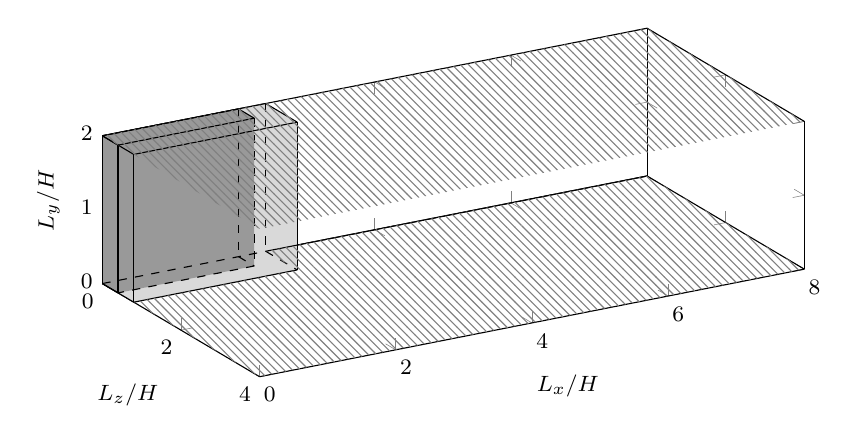
\begin{tikzpicture}
\pgfplotsset{
    scale only axis,
}
\begin{axis}[
view={-30}{20},
		xlabel={$L_x/H$},
		ylabel={$L_z/H$},
		zlabel={$L_y/H$},
		unit vector ratio=1 1 1,
		xmin=0,xmax=8,
		ymin=0,ymax=4,
		zmin=0,zmax=2,
		y dir=reverse,
		clip=true,
		set layers,
		clip mode=individual,
		height=.7\textwidth,
		width=.9\textwidth,
		xtick={0,2,...,8},
		ytick={0,2,...,4},
		ztick={0,1,2},
		label style={font=\footnotesize},
		tick label style={font=\footnotesize},
	]
	\pgfmathparse{atan(tan(-50)*sin(70))}
  \let\a=\pgfmathresult
  \pgfmathparse{atan(tan(90+50)*sin(70))}
  \let\b=\pgfmathresult  

	\centering
%\addplot3 [thick, color=blue, on layer=axis background]
%graphics[xmin=0,ymin=0,xmax=8,ymax=4,zmin=0,zmax=0]{Figures/G24Fc.png};

\fill[color=gray!30,opacity=100] (0,0.8,0) -- (2.4,0.8,0) -- (2.4,0.8,2) -- (0,0.8,2) -- cycle;
\fill[color=gray!30,opacity=100] (0,0,0) -- (0,0.8,0) -- (0,0.8,2) -- (0,0,2) -- cycle;
\fill[color=gray!30,opacity=100] (0,0,2) -- (0,0.8,2) -- (2.4,0.8,2) -- (2.4,0,2) -- cycle;
\fill[color=gray!80,opacity=100] (0,0.4,0) -- (2,0.4,0) -- (2,0.4,2) -- (0,0.4,2) -- cycle;
\fill[color=gray!80,opacity=100] (0,0,0) -- (0,0.4,0) -- (0,0.4,2) -- (0,0,2) -- cycle;
\fill[color=gray!80,opacity=100] (0,0,2) -- (0,0.4,2) -- (2,0.4,2) -- (2,0,2) -- cycle;
\draw[-,black] (2.4,0,0) -- (8,0,0);

%\draw[-,black] (0,0,0) -- (2,0,0);
\draw[-,dashed,black] (2,0,0) -- (2,0.4,0);
\draw[-,dashed,black] (2,0.4,0) -- (0,0.4,0);
\draw[-,black] (0,0.4,0) -- (0,0,0);


\draw[-,black] (0,0,2) -- (2,0,2);
\draw[-,black] (2,0,2) -- (2,0.4,2);
\draw[-,black] (2,0.4,2) -- (0,0.4,2);
\draw[-,black] (0,0.4,2) -- (0,0,2);

\draw[-,black] (0,0,2) -- (0,0,0);
\draw[-,dashed,black] (2,0,2) -- (2,0,0);
\draw[-,dashed,black] (2.4,0,2) -- (2.4,0,0);
\draw[-,black] (2.4,0.8,2) -- (2.4,0.8,0);
\draw[-,dashed,black] (2,0.4,2) -- (2,0.4,0);
\draw[-,black] (0,0.4,2) -- (0,0.4,0);
\draw[-,black] (0,0.8,2) -- (0,0.8,0);

\draw[-,dashed,black] (0,0,0) -- (2.4,0,0);
\draw[-,dashed,black] (2.4,0,0) -- (2.4,0.8,0);
\draw[-,black] (2.4,0.8,0) -- (0,0.8,0);
\draw[-,black] (0,0.8,0) -- (0,0,0);


\draw[-,black] (0,0,2) -- (2.4,0,2);
\draw[-,black] (2.4,0,2) -- (2.4,0.8,2);
\draw[-,black] (2.4,0.8,2) -- (0,0.8,2);
\draw[-,black] (0,0.8,2) -- (0,0,2);

\fill[pattern=north west lines, pattern color=gray] (0,0.8,0) -- (8,0.8,0) -- (8,4,0) -- (0,4,0) -- cycle;
\fill[pattern=north west lines, pattern color=gray] (2.4,0,0) -- (8,0,0) -- (8,0.8,0) -- (2.4,0.8,0) -- cycle;
\fill[pattern=north west lines, pattern color=gray] (0,0,2) -- (8,0,2) -- (8,4,2) -- (0,4,2) -- cycle;
%graphics[xmin=0,ymin=0,xmax=8,ymax=4,zmin=0,zmax=0]{Figures/G24Fc.png};
%\node[gray,left] at (axis cs: 2,0.2,0) {\tiny$M2$};
%\node[gray,left] at (axis cs: 2.4,0.6,0) {\tiny$M1$};
%\node[gray,left] at (axis cs: 8,3.8,0) {\tiny$F$};
\end{axis}
\end{tikzpicture}
%\caption{Schematic of full-span channel and minimal channels, roughness on upper boundary is not shown.}
%\end{subfigure}
%\begin{subfigure}[c]{.49\linewidth}
%\begin{tikzpicture}
\pgfplotsset{
    scale only axis,
}
\begin{axis}[
		xlabel={$L_x/H$},
		ylabel={$L_z/H$},
		unit vector ratio=1 1 1,
		xmin=0,xmax=8,
		ymin=0,ymax=4,
		y dir=reverse,
		clip=true,
		set layers,
		clip mode=individual,
		width=.7\textwidth,
		xtick={0,2,...,8},
		ytick={0,2,...,4},
		label style={font=\footnotesize},
		tick label style={font=\footnotesize},
		colorbar,
		point meta min=0,
		point meta max=0.1226,
		colorbar style={
			xlabel={$k/H$},
			xlabel shift = 10.5 pt,
		ytick={0,0.12},
		width=0.2cm
		}
	]
	\centering
\addplot [thick, color=blue, on layer=axis background]
graphics[xmin=0,ymin=0,xmax=8,ymax=4]{Figures/G24Fc.png};
\draw[color=black,thick] (0, 0) rectangle (2, 0.4);
\draw[color=black,thick] (0, 0) rectangle (2.4, 0.8);
\node[black,left] at (axis cs: 2,0.2) {\textbf{$M$2-500}};
\node[black,left] at (axis cs: 2.4,0.6) {\textbf{$M$1-500}};
\node[black,left] at (axis cs: 8,3.8) {\textbf{$F$-500}};
\end{axis}
\end{tikzpicture}
%\caption{Roughness map of G24F}
%\end{subfigure}
%\caption {Comparison of channel sizes, black frames indicate minimal channels \textit{M1}\& \textit{M2}}
%\label{G24F}
%\end{figure}
%\begin{figure}[H]
%	\begin{subfigure}[t]{.5\textwidth}
%	\centering
%	        \begin{tikzpicture}[]
        \centering
        \begin{axis}[
            ylabel={$U^+$},
            xlabel={$(y-d)^+$},
            ymin=0, ymax=30,
			xmin=1,xmax=500,
            width=1.05\textwidth,
            height=0.8\textwidth,
			xmode=log,
            legend style={fill=white,font=\tiny,anchor=north west},
            legend pos=north west,
            label style={font=\footnotesize},
            tick label style={font=\footnotesize}
            ]
            \addplot [
            black,dashed,thick,
            ]
            table [x=X, y=Y,col sep=comma]{CSV/UprofileG24FM1.csv};
            \addlegendentry{critical height $y_c$}
            			            \addplot [
            gray!50,solid,thick,
            ]
            table [x=X, y=Y,col sep=comma]{CSV/G24M31.csv};
            \addlegendentry{$G24M3-500$}
			            \addplot [
            red,solid,thick,
            ]
            table [x=X, y=Y,col sep=comma]{CSV/UprofileG24FM6.csv};
            \addlegendentry{$G24M2-500$}
			\addplot [
            green,solid,thick,
            ]
            table [x=X, y=Y,col sep=comma]{CSV/UprofileG24FM7.csv};
            \addlegendentry{$G24M1-500$}
						\addplot [
            blue,solid,thick,
            ]
            table [x=X, y=Y,col sep=comma]{CSV/UprofileG24FM8.csv};
            \addlegendentry{$G24F-500$}
						\addplot [
            black,dashdotted,thick,
            ]
            table [x=X, y=Y,col sep=comma]{CSV/UprofileG24FM9.csv};
            \addlegendentry{$U^+=(\frac{1}{0.4})\text{log}(y^+)+5.2$}
            \draw [dashdotted,red, thick] (50-45.80,0) -- (50-45.80,30);
            \addplot [
            black,dashed,thick,
            ]
            table [x=X, y=Y,col sep=comma]{CSV/UprofileG24FM2.csv};
            \addplot [
            blue,dashed,thick,
            ]
            table [x=X, y=Y,col sep=comma]{CSV/UprofileG24FM3.csv};
            \addplot [
            green,dashed,thick,
            ]
            table [x=X, y=Y,col sep=comma]{CSV/UprofileG24FM4.csv};	            
\addplot [
            red,dashed,thick,
            ]
            table [x=X, y=Y,col sep=comma]{CSV/UprofileG24FM5.csv};
\draw [dashed,gray!50] (60,0) -- (60,30);

        \end{axis}
        \end{tikzpicture}
%	\caption{Mean velocity profile of case \textit{G24}\\(\full: Rough, \dashed: smooth)}
%	\end{subfigure}
%	\begin{subfigure}[t]{.5\textwidth}
%	\centering
%	        \begin{tikzpicture}[]
        \centering
        \begin{axis}[
            ylabel={$\Delta U^+$},
            xlabel={$(y-d)^+$},
            ymin=-2, ymax=8,
			xmin=1,xmax=500,
            width=1.05\textwidth,
            height=0.8\textwidth,
			xmode=log,
            legend style={font=\tiny,anchor=south east},
            legend pos= south east,
            label style={font=\footnotesize},
            tick label style={font=\footnotesize}
            ]
            \addplot [
            black,dashed,thick,
            ]
            coordinates{
            (160, 10)
            (160, -5)
            };
            \addlegendentry{critical height $y_c$}
						\addplot [
            red,solid,thick,
            ]
            table [x=X, y=Y,col sep=comma]{CSV/DUprofileG24mf23.csv};
            \addlegendentry{$G24M2-500$}
									\addplot [
            green,solid,thick,
            ]
            table [x=X, y=Y,col sep=comma]{CSV/DUprofileG24mf24.csv};
            \addlegendentry{$G24M1-500$}
						\addplot [
            blue,solid,thick,
            ]
            table [x=X, y=Y,col sep=comma]{CSV/DUprofileG24mf25.csv};
            \addlegendentry{$G24F-500$}
                        \draw [dashdotted,red, thick] (50-45.80,-8) -- (50-45.80,30);
            \addplot [
            black,dashed,thick,
            ]
            coordinates{
            (80, 10)
            (80, -5)
            };


        \end{axis}
        \end{tikzpicture}
%	\caption{Velocity offset profile of case \textit{G24}}
%	\end{subfigure}
%\caption{Results from \textit{G24}. Red: $M2$, green: $M1$, blue: $F$}
%\label{UG24}
%\end{figure}
\begin{table}[H]
\centering
\caption{Summary of roughness function $\Delta U^+$ at $Re_\tau\approx500$, marked values are taken as the minimal channel results}
    \begin{tabular}{|c| c c c |c|c c c|}
    \hline
     Case&\textit{F}&\textit{M1}&\textit{M2}& Case&\textit{F}&\textit{M1}&\textit{M2} \\
     \hline
	\hline
     \textit{G14}&6.7&6.7&\textbf{6.6}&\textit{G24}&6.3&6.4&\textbf{6.2}\\ 
    \textit{G18}&6.6&\textbf{6.6}&-&\textit{G28}&5.9&\textbf{5.9}&-\\
    \hline
    \textit{P14}&7.3&7.3&\textbf{7.4}&\textit{P24}&7.0&6.9&\textbf{6.9}\\
    \textit{P18}&7.2&\textbf{7.3}&-&\textit{P28}&6.6&\textbf{6.6}&-\\
    \hline
    \textit{N14}&6.1&6.1&\textbf{5.9}&\textit{N24}&5.8&5.6&\textbf{5.8}\\
    \textit{N18}&6.1&\textbf{6.1}&-&\textit{N28}&5.5&\textbf{5.6}&-\\
    \hline
    \end{tabular}
\label{ResultAll}
\end{table}
\begin{figure}[H]
    \centering
            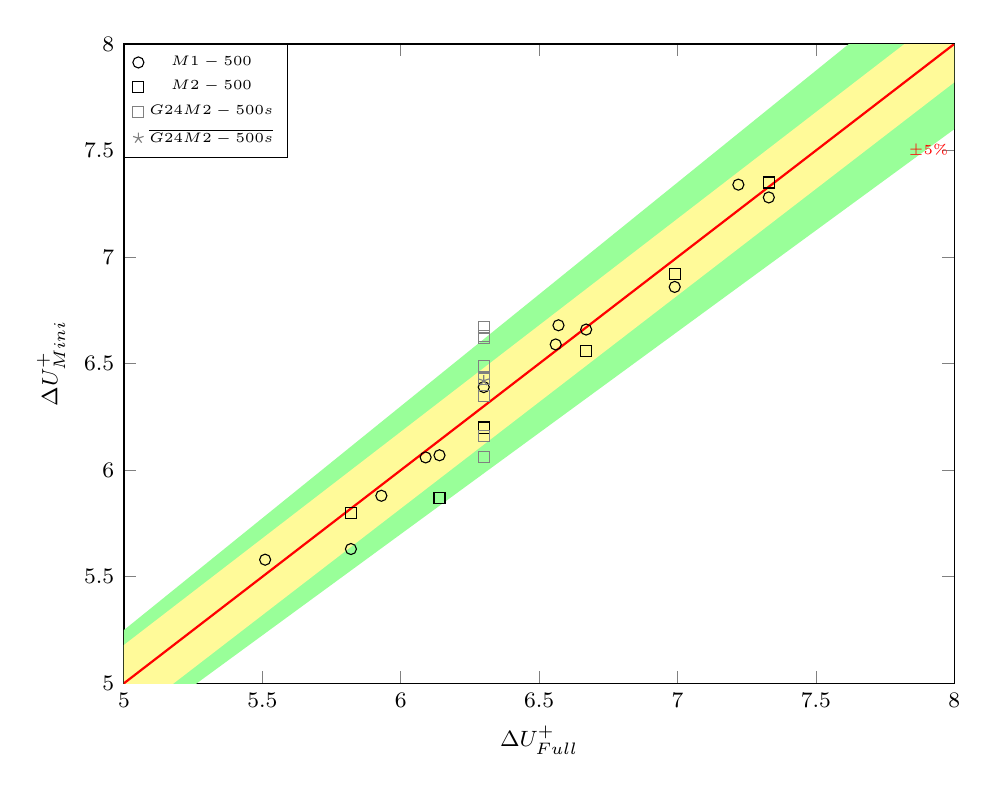
\begin{tikzpicture}[]
        \centering
        \begin{axis}[
            ylabel={$\Delta U_{Mini}^+$},
            xlabel={$\Delta U_{Full}^+$},
            ymin=5, ymax=8,
			xmax=8,
			xmin=5,
			%xtick={-2,-1.5,...,-0.4},
            width=1\linewidth,
            height=.8\linewidth,
            label style={font=\footnotesize},
			legend style={font=\tiny,at={(0,1)},anchor=north west},
            tick label style={font=\footnotesize}
            ]
			\addplot [
            black,only marks,mark=o,
            ]
            coordinates{
            (6.67, 6.66)
            (6.56, 6.59)
            (6.30,6.39)
            (5.93,5.88)
            (7.33,7.28)
            (7.22,7.34)
            (6.99,6.86)
            (6.57,6.68)
            (6.14,6.07)
            (6.09,6.06)
            (5.82,5.63)
            (5.51,5.58)
            };
			\addlegendentry{$M1-500$}
			\addplot [
            black,only marks,mark=square,
            ]
            coordinates{
            (6.67, 6.56)
            (6.30, 6.20)
            (7.33,7.35)
            (6.99,6.92)
            (6.14,5.87)
            (5.82,5.80)
            };
			\addlegendentry{$M2-500$}
						\addplot [
            gray,only marks,mark=square,
            ]
            coordinates{
            (6.30, 6.06)
            (6.30, 6.43)
            (6.30, 6.35)
            (6.30, 6.49)
            (6.30, 6.62)
            (6.30, 6.67)
            (6.30, 6.63)
            (6.30, 6.16)
            };
			\addlegendentry{$G24M2-500s$}
									\addplot [
            gray,only marks,mark=star,
            ]
            coordinates{
            (6.30, 6.42)
            };
			\addlegendentry{$\overline{G24M2-500s}$}
			 \fill[color=green!40,opacity=40] (0,0) -- (9,9.45) -- (9,8.55) -- cycle;
			 			\fill[color=yellow!40,opacity=40] (0,0.18) -- (9,9.18) -- (9,8.82) -- (0,-0.18) -- cycle;
						\addplot [
            red,thick,solid,mark=square,
            ]
            coordinates{
            (0, 0)
            (9, 9)
            };
			\node[red,right] at (axis cs: 7.8,7.5) {\tiny $\pm5\%$};
        \end{axis}
        \end{tikzpicture}
    \caption{$\Delta U^+$ predicted by minimal channels against prediction by full span channel, $\Delta$: minimal channel $M1$, $\square$: minimal channel $M2$. Green shadow indicates prediction error interval of $\pm5\%$ around $\Delta U_{Full}^+=\Delta U_{Mini}^+$ (\Rfull)}
    \label{DUfullmini}
\end{figure}
\subsubsection{Effect of random process}
\label{Rando}
Due to the random nature of the roughness generation process, bias of statistics are expected on limited population of samples.
In present section the prediction error caused by the random generation process is studied.
To this end, ten rough surfaces corresponding to the configuration G24M2 are generated independently.
Resulting roughness maps are shown in Fig.~\ref{ten}.
The predictions of $\Delta U^+$ at $Re_\tau=500$ are summarized in table~\ref{tab:ten}.
%A kernel density estimation with bandwidth$=0.15$ is applied, single peak pdf profile is obtained as shown in Fig.~\ref{PDFG24s}.
The mean value of roughness function $\overline{\Delta U}^+=6.53$ with 95\% uncertainty interval of 0.34.
Therefore a narrow uncertainty interval due to the random process is detected for simulation case $G24M2$.
%\begin{figure}[H]
%\begin{subfigure}[t]{0.5\linewidth}
%\centering
%\input{tikz/1.tikz}

%\caption{\textit{G24M2.1}}
%\end{subfigure}\hfill%
%\begin{subfigure}[t]{0.5\linewidth}
%\centering
%\input{tikz/2.tikz}
%\vspace{-0.5cm}

%\caption{\textit{G24M2.2}}
%\end{subfigure}
%\begin{subfigure}{0.5\linewidth}
%\centering
%\begin{tikzpicture}
\begin{axis}[
		xlabel=$L_x$,
		ylabel=$L_z$,
		xmin=0,xmax=2.0,
		ymin=0,ymax=0.4,
		y dir=reverse,
		clip=true,
		set layers,
		clip mode=individual,
		height=0.34\linewidth,
		width=.83\linewidth,
		xtick={0,0.4,...,2.0},
		ytick={0,0.2,...,0.4},
		label style={font=\footnotesize},
		tick label style={font=\footnotesize},
	]
	\centering
\addplot [thick, color=blue, on layer=axis background]
graphics[xmin=0,ymin=0,xmax=2.0,ymax=0.4]{Figures/3.png};

\end{axis}
\end{tikzpicture}
%\caption{\textit{G24M2.3}}
%\end{subfigure}\begin{subfigure}{0.5\linewidth}
%\centering
%\input{tikz/4.tikz}
%\vspace{-0.5cm}
%\caption{\textit{G24M2.4}}
%\end{subfigure}
%\begin{subfigure}{0.5\linewidth}
%\centering
%\input{tikz/5.tikz}
%\caption{\textit{G24M2.5}}
%\end{subfigure}\begin{subfigure}{0.5\linewidth}
%\centering
%\input{tikz/6.tikz}
%\vspace{-0.5cm}
%\caption{\textit{G24M2.6}}
%\end{subfigure}
%\begin{subfigure}{0.5\linewidth}
%\centering
%\input{tikz/7.tikz}
%\caption{\textit{G24M2.7}}
%\end{subfigure}\begin{subfigure}{0.5\linewidth}
%\centering
%\input{tikz/8.tikz}
%\vspace{-0.5cm}
%\caption{\textit{G24M2.8}}
%\end{subfigure}
%\begin{subfigure}{0.5\linewidth}
%\centering
%\input{tikz/9.tikz}
%\caption{\textit{G24M2.9}}
%\end{subfigure}\begin{subfigure}{0.5\linewidth}
%\centering
%\input{tikz/10.tikz}
%\vspace{-0.5cm}
%\caption{\textit{G24M2.10}}
%\end{subfigure}
%\caption{Roughness maps of ten \textit{G24M2}s}
%\label{ten}
%\end{figure}
\begin{table}[H]
    \centering
        \caption{Roughness function of G24M2s}
    \begin{tabular}{|c c| c c|}
    \hline
         Case& $\Delta U^+$ &Case& $\Delta U^+$  \\
         \hline
         1 & 6.06& 6 &6.67\\
         2&6.43&7&6.97\\
         3&6.35&8&6.63\\
         4&6.49&9&6.82\\
         5&6.78&10&6.16\\
         \hline
    \end{tabular}

    \label{tab:ten}
\end{table}
%\begin{figure}[H]
%    \centering
%    \begin{tikzpicture}[]
        \centering
        \begin{axis}[
            ylabel={Possibility density},
            xlabel={$\Delta U^+$},
            %ymin=0, ymax=1,
			%xmin=2,xmax=200,
            width=.5\textwidth,
            height=.5\textwidth,
			%xmode=log,
            %legend style={font=\tiny,at={(axis cs:9,-1)},anchor=south west},
            %legend style={fill=none,font=\tiny,at={(0,1)},anchor=north west},
            label style={font=\footnotesize},
            tick label style={font=\footnotesize}
            ]
            \addplot [
            black,solid,thick,
            ]
            table [x=X, y=Y,col sep=comma]{CSV/PDFG241.csv};
            \draw[<->] (6.33,0) -- (6.73,0);
            %\addlegendentry{Industrial pipe~\cite{Moody1944}}
        \end{axis}
        \end{tikzpicture}
%    \caption{PDF estimation of $\Delta U^+$}
%    \label{PDFG24s}
%\end{figure}
\subsubsection{Minimal channel simulation of different flow regime}
\label{Res}
Surface $G24$ is evaluated in different $Re_\tau\approx250-1000$, both minimal channel simulations $M2\&M1$ as well as large-span channel simulations $F/M0$ are carried out. 
Simulation setups are summarized in table~\ref{tab:Re}.
Mean velocity profiles are shown in Fig.~\ref{Re_expand}(a), while roughness functions $\Delta U^+$ against $k^+$ are shown in Fig.~\ref{Re_expand}(b). 
In Fig.~\ref{Re_expand}(a) minimal channels $M2$ are plotted with dotted lines, $M1$ are plotted with dashed line while (pseudo) full span channels $F/M0$ are plotted with solid lines.
One can observe from Fig.~\ref{Re_expand}(a) that each velocity profiles deviate above respective critical height $y_c^+=0.4\times L_z^+$ which are not shown for simplicity. 
By subtracting velocity profile from the log-law $$U^+=\frac{1}{\kappa}\text{log}(y^+)+5.2$$ roughness functions are obtained at each critical height.
By fitting roughness function to the asymptotic line, equivalent sand-grain size of $G24$ is estimated $k_s\approx 1.15\times k$.
Roughness function is shown in Fig.~\ref{Re_expand}(b) as a function of equivalent sand-grain size $k_s^+$. 
It can be observed that $\Delta U^+$ asymptotically approaches fully rough regime at $k^+=50$, it is believed that roughness is in fully rough regime at such roughness Reynolds number.
\begin{figure}[H]
    \centering
    \begin{subfigure}[t]{.49\linewidth}
                \begin{tikzpicture}[]
        \centering
        \begin{axis}[
            ylabel={$U^+$},
            xlabel={$(y-d)^+$},
            %ymin=0, ymax=1,
            ymax=30,
			xmin=1,xmax=1000,
            width=1.05\textwidth,
            height=1\textwidth,
			xmode=log,
            %legend style={font=\tiny,at={(axis cs:9,-1)},anchor=south west},
            legend style={fill=white,font=\tiny,anchor=north west},
            label style={font=\footnotesize},
            legend pos=north west,
            tick label style={font=\footnotesize}
            ]
            %\addplot [
            %black!25,dashed,thick,
            %]
            %table [x=X, y=Y,col sep=comma]{CSV/Reall1.csv};
            %\addlegendentry{1}
            %\addplot [
            %black!100,dashed,thick,
            %]
            %table [x=X, y=Y,col sep=comma]{CSV/Reall2.csv};
            %\addlegendentry{2}
            %            \addplot [
            %black!75,dashed,thick,
            %5]
            %table [x=X, y=Y,col sep=comma]{CSV/Reall3.csv};
            %\addlegendentry{3}
            %            \addplot [
            %black!50,dashed,thick,
            %]
            %table [x=X, y=Y,col sep=comma]{CSV/Reall4.csv};
            %\addlegendentry{4}
                        \addplot [
            black!100,solid,thick,
            ]
            table [x=X, y=Y,col sep=comma]{CSV/Reall5.csv};
            \addlegendentry{$Re_\tau=1000$, $k^+=100$}
                        \addplot [
            black!75,solid,thick,
            ]
            table [x=X, y=Y,col sep=comma]{CSV/Reall6.csv};
            \addlegendentry{$Re_\tau=750$, $k^+=75$}
                        \addplot [
            black!50,solid,thick,
            ]
            table [x=X, y=Y,col sep=comma]{CSV/Reall7.csv};
            \addlegendentry{$Re_\tau=500$, $k^+=50$}
                        \addplot [
            black!25,solid,thick,
            ]
            table [x=X, y=Y,col sep=comma]{CSV/Reall18.csv};
            \addlegendentry{$Re_\tau=250$, $k^+=25$}
                        \addplot [
            black,densely dashed,thin,
            ]
            table [x=X, y=Y,col sep=comma]{CSV/Reall9.csv};
            \addlegendentry{$U^+=(\frac{1}{0.4})\text{log}(y^+)+5.2$}
                        \addplot [
            black!100,dashed,thick,
            ]
            table [x=X, y=Y,col sep=comma]{CSV/Reall10.csv};
                        \addplot [
            black!75,dashed,thick,
            ]
            table [x=X, y=Y,col sep=comma]{CSV/Reall11.csv};
                        \addplot [
            black!50,dashed,thick,
            ]
            table [x=X, y=Y,col sep=comma]{CSV/Reall12.csv};
                        \addplot [
            black!25,dashed,thick,
            ]
            table [x=X, y=Y,col sep=comma]{CSV/Reall13.csv};
                        \addplot [
            black!100,dotted,thick
            ]
            table [x=X, y=Y,col sep=comma]{CSV/Reall15.csv};
                        \addplot [
            black!75,dotted,thick
            ]
            table [x=X, y=Y,col sep=comma]{CSV/Reall16.csv};
                        \addplot [
            black!50,dotted,thick
            ]
            table [x=X, y=Y,col sep=comma]{CSV/Reall17.csv};
                        \addplot [
            black!25,dotted,thick
            ]
            table [x=X, y=Y,col sep=comma]{CSV/Reall8.csv};
%            \draw [solid,red] (25-23.1,2.9) -- (25-23.1,3.9);
%            \draw [solid,red] (50-45.8,2) -- (50-45.8,3);
%             \draw [solid,red] (75-65.7,2) -- (75-65.7,2.9);
%             \draw [solid,red] (100-86.4,1.7) -- (100-86.4,2.7);
        \end{axis}
        \end{tikzpicture}
    \caption{Mean velocity profiles at $Re_\tau=250-1000$, line color gradually changes from gray to black with increasing $Re_\tau$.\\(\full: $F/M0$, \dashed: $M1$, \dotted: $M2$)}
    \end{subfigure}\hfill%
    \begin{subfigure}[t]{.49\linewidth}
                \begin{tikzpicture}[]
        \centering
        \begin{axis}[
            ylabel={$\Delta U^+$},
            xlabel={$k_s^+$},
            %ymin=0, ymax=1,
			xmin=2,xmax=200,
            width=1.05\textwidth,
            height=1\textwidth,
			xmode=log,
            %legend style={font=\tiny,at={(axis cs:9,-1)},anchor=south west},
            legend style={fill=none,font=\tiny,anchor=north west},
            legend pos=north west,
            label style={font=\footnotesize},
            tick label style={font=\footnotesize}
            ]
            \addplot [
            black,dashed,thick,
            ]
            table [x=x, y=Curve1,col sep=comma]{CSV/IndustrialPipe.csv};
            \addlegendentry{\citet{Moody1944}}
						\addplot [
            black,only marks,mark=x,
            ]
            table [x=x, y=Curve1,col sep=comma]{CSV/Nikuradse.csv};
            \addlegendentry{\citet{Nikuradse1933}}
			\addplot [
            blue,only marks,mark=triangle,
            ]
            coordinates{
            (25*1.05, 3.3004)
            (50*1.05, 6.5559)
            (75*1.05,7.5656)
            (100*1.05,8.5828)
            };
			\addlegendentry{$F/M0$}
						\addplot [
            green,only marks,mark=square,
            ]
            coordinates{
            (25*1.05, 3.0168)
            (50*1.05, 6.4357)
            (75*1.05,7.8237)
            (100*1.05,8.7559)
            };
			\addlegendentry{$M1$}
									\addplot [
            red,only marks,mark=o,
            ]
            coordinates{
            (25*1.05, 3.2272)
            (50*1.05, 6.3661)
            (75*1.05,7.7649)
            (100*1.05,8.9487)
            };
			\addlegendentry{$M2$}
        \end{axis}
        \end{tikzpicture}
    \caption{Roughness function $\Delta U^+(k_s^+)$. Data from Nikuradse's uniform sand grain roughness and Colebrook relation for industrial pipes are added for comparison.}
    \end{subfigure}
    \caption{Simulation of different $Re_\tau$}
    \label{Re_expand}
\end{figure}
%\begin{figure}
%    \centering
%    \begin{subfigure}{0.49\linewidth}
%    \input{tikz/Re_250}
%    \caption{250}
%    \end{subfigure}
%        \begin{subfigure}{0.49\linewidth}
%    \input{tikz/Re_750}
%    \caption{750}
%    \end{subfigure}
%        \begin{subfigure}{0.49\linewidth}
%            \begin{tikzpicture}[]
        \centering
        \begin{axis}[
            ylabel={$U^+$},
            xlabel={$(y-y_0)^+$},
            %ymin=0, ymax=1,
			xmin=1,xmax=1000,
            width=1\textwidth,
            height=.8\textwidth,
			xmode=log,
            %legend style={font=\tiny,at={(axis cs:9,-1)},anchor=south west},
            legend style={font=\tiny,at={(1,0)},anchor=south west},
            label style={font=\footnotesize},
            tick label style={font=\footnotesize}
            ]
                                    \addplot [
            gray,dashed,thin,
            ]
            table [x=X, y=Y,col sep=comma]{CSV/Reall9.csv};
            \addlegendentry{Log law}

                        \addplot [
            black,solid,thick,
            ]
            table [x=X, y=Y,col sep=comma]{CSV/Reall5.csv};
            \addlegendentry{$F$}

                        \addplot [
            black,dashed,thick,
            ]
            table [x=X, y=Y,col sep=comma]{CSV/Reall10.csv};
            \addlegendentry{$M1$}
                        \addplot [
            black,dash dot,thick
            ]
            table [x=X, y=Y,col sep=comma]{CSV/Reall15.csv};
            \addlegendentry{$M2$}
                        \addplot [
            black!25,dashed,thick,
            ]
            table [x=X, y=Y,col sep=comma]{CSV/Reall2.csv};
            \addlegendentry{Critical height $y_c$}
        \end{axis}
        \end{tikzpicture}
%    \caption{1000}
%    \end{subfigure}
%    \caption{Caption}
%    \label{fig:my_label}
%\end{figure}
\subsection{Effect roughness geometry}
\label{results}
 Since the capability of the minimal channel is demonstrated, following analysis will be carried out basing on the results from minimal channels.
 Due to the different settings of $\lambda_0$, $M2$ is regarded as the minimal channel for cases with $\lambda_0=0.4H$, while for cases with $\lambda_0=0.8H$, $M1$ is used. 
 Therefore, the marked values in table~\ref{ResultAll} are regarded as minimal channel results and will be used in this section.\\
 
 An overview of the results from minimal channels are plotted in Fig.~\ref{fig:3d}(a), where roughness function $\Delta U^+$ is shown as a function of two of the concerned roughness parameters, i.e. Skewness $Sk$ and PS slope $p$.
 Color indicates different $\lambda_0$, black: $\lambda_0=0.4H$, gray: $\lambda_0=0.8H$.
 In order to isolate the effect of each roughness parameter of interest, roughness functions from Fig.~\ref{fig:3d}(a) are plotted against each of the variables i.e. $Sk$, $p$ and $\lambda_0$ respectively in Fig.\ref{fig:3d}(b,c,d).
\begin{figure}
    \hspace{-1.5cm}
    \begin{tikzpicture}
\node (overview) at (-10,5) {        \begin{tikzpicture}[]
        \centering
        \begin{axis}[
        view={40}{35},
            ylabel={$p$},
            xlabel={$Sk$},
			zlabel={$\Delta U^+$},
			ztick={5.5,6,6.5,7,7.5},
            %ymin=0, ymax=1,
            width=.6\textwidth,
            height=.4\textwidth,
            label style={font=\footnotesize},
            tick label style={font=\footnotesize}
            ]
 %           \addplot3 [
%            blue,dashed,thick,no marks
%            ]
%            coordinates{
%            (0,-2,6.326)			%
%			(0.48,-2,6.994)%
%			(0.48,-1,7.336)
%			(0,-1,6.656)
%			(-0.48,-1,6.096)
%			(-0.48,-2,5.789)
 %           (0,-2,6.326)
%			};
%			\addplot3 [
 %5           red,dashed,thick, no marks
  %          ]
   %         coordinates{
    %        
    % 5       (0,-2,5.912)
	%		(0.48,-2,6.607)
	%		(0.48,-1,7.262)
	%5		(0,-1,6.530)
	%5		(-0.48,-1,6.075)
	%		(-0.48,-2,5.458)
	%5		(0,-2,5.912)
     %       };
                        \addplot3 [
            black,mark=x,thick, mark size=3pt
            ]
            coordinates{
            (0,-2,6.20)			
			(0.48,-2,6.9176)
			(0.48,-1,7.3502)
			(0,-1,6.56)
			(-0.48,-1,5.87)
			(-0.48,-2,5.8034)
            (0,-2,6.20)
			};
			\addplot3 [
            gray!60,mark=x,thick, mark size=3pt
            ]
            coordinates{
            
            (0,-2,5.8764)
			(0.48,-2,6.8720)
			(0.48,-1,7.3415)
			(0,-1,6.5891)
			(-0.48,-1,6.0625)
			(-0.48,-2,5.5765)
			(0,-2,5.8764)
            };
                                    \addplot3 [
            black,mark=x,thick, mark size=3pt
            ]
            coordinates{
            (0,-2,6.20)			
			(0,-1,6.56)
			};
			\addplot3 [
            gray!60,mark=x,thick, mark size=3pt
            ]
            coordinates{
            (0,-2,5.8764)
			(0,-1,6.5891)
            };
        \end{axis}
        \end{tikzpicture}};
\node (caption_overview) [right=of overview,align=left] {(a) Overview of results.\\Black: $\lambda_0=0.8H$, gray: $\lambda_0=1.6H$};
\node (Sk) at (-15,0) {        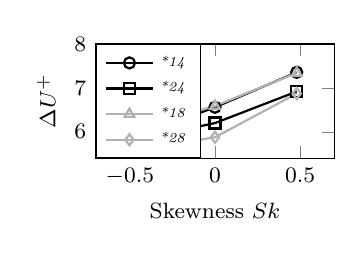
\begin{tikzpicture}[]
        \centering
        \begin{axis}[
            ylabel={$\Delta U^+$},
            xlabel={Skewness $Sk$},
            ymin=5.4, ymax=8,
			xmax=0.7,
			xmin=-0.7,
            width=.38\textwidth,
            height=.25\textwidth,
            label style={font=\footnotesize},
			legend style={font=\tiny,at={(0,1)},anchor=north west},
            tick label style={font=\footnotesize}
            ]
			\addplot [
            black,solid,thick,mark=o,
            ]
            coordinates{
            (-0.48, 5.87)
            (0, 6.56)
            (0.48, 7.3562)
            };
			\addlegendentry{\textit{*14}}
			\addplot [
            black,solid,thick,mark=square,
            ]
            coordinates{
            (-0.48, 5.8034)
            (0, 6.20)
            (0.48, 6.9176)
            };
			\addlegendentry{\textit{*24}}
			\addplot [
            gray!60,solid,thick,mark=triangle,
            ]
            coordinates{
            (-0.48, 6.0625)
            (0, 6.5891)
            (0.48, 7.3415)
            };
			\addlegendentry{\textit{*18}}
						\addplot [
            gray!60,solid,thick,mark=diamond,
            ]
            coordinates{
            (-0.48, 5.5765)
            (0, 5.8764)
            (0.48, 6.8720)
            };
			\addlegendentry{\textit{*28}}
        \end{axis}
        \end{tikzpicture}};
\node (caption_sk) [below=of Sk,align=left] {(b) $\Delta U^+$ as a function of $Sk$.\\Black: $\lambda_0=0.8H$, gray: $\lambda_0=1.6H$};
\node (p) at (-5,0) {        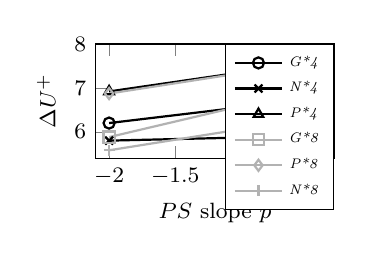
\begin{tikzpicture}[]
        \centering
        \begin{axis}[
            ylabel={$\Delta U^+$},
            xlabel={$PS$ slope $p$},
            ymin=5.4, ymax=8,
			xmax=-0.3,
			xmin=-2.1,
			xtick={-2,-1.5,...,-0.4},
            width=.38\textwidth,
            height=.25\textwidth,
            label style={font=\footnotesize},
			legend style={font=\tiny,at={(1,1)},anchor=north east},
            tick label style={font=\footnotesize}
            ]
			\addplot [
            black,solid,thick,mark=o,
            ]
            coordinates{
            (-1, 6.56)
            (-2, 6.20)
            };
			\addlegendentry{\textit{G*4}}
			
									\addplot [
           black,solid,thick,mark=x,
            ]
            coordinates{
            (-1, 5.87)
            (-2, 5.80)
            };
			\addlegendentry{\textit{N*4}}
									\addplot [
           black,solid,thick,mark=triangle,
            ]
            coordinates{
            (-1, 7.3562)
            (-2, 6.92)
            };
			\addlegendentry{\textit{P*4}}
			
			\addplot [
            gray!60,solid,thick,mark=square,
            ]
            coordinates{
            (-1, 6.59)
            (-2, 5.88)
            };
			\addlegendentry{\textit{G*8}}

						\addplot [
            gray!60,solid,thick,mark=diamond,
            ]
            coordinates{
            (-1, 7.34)
            (-2, 6.8720)
            };
			\addlegendentry{\textit{P*8}}

						\addplot [
            gray!60,solid,thick,mark=+,
            ]
            coordinates{
            (-1, 6.06)
            (-2, 5.58)
            };
			\addlegendentry{\textit{N*8}}
        \end{axis}
        \end{tikzpicture}};
\node (caption_p) [below=of p,align=left] {(c) $\Delta U^+$ as a function of $p$.\\Black: $\lambda_0=0.8H$, gray: $\lambda_0=1.6H$};
\node (lambda) at (-10.5,-6.5) {        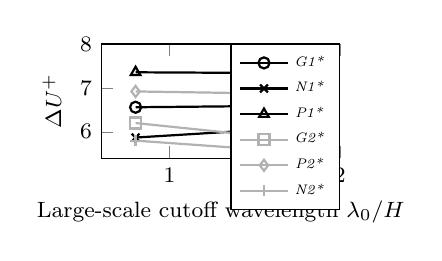
\begin{tikzpicture}[]
        \centering
        \begin{axis}[
            ylabel={$\Delta U^+$},
            xlabel={Large-scale cutoff wavelength $\lambda_0/H$},
            ymin=5.4, ymax=8,
			xmax=2,
			xmin=0.6,
            width=.38\textwidth,
            height=.25\textwidth,
            label style={font=\footnotesize},
			legend style={font=\tiny,at={(1,1)},anchor=north east},
            tick label style={font=\footnotesize}
            ]
			\addplot [
            black,solid,thick,mark=o,
            ]
            coordinates{
            (0.8, 6.56)
            (1.6, 6.59)
            };
			\addlegendentry{\textit{G1*}}
			
									\addplot [
            black,solid,thick,mark=x,
            ]
            coordinates{
            (0.8, 5.87)
            (1.6, 6.06)
            };
			\addlegendentry{\textit{N1*}}
			
						\addplot [
            black,solid,thick,mark=triangle,
            ]
            coordinates{
            (0.8, 7.3562)
            (1.6, 7.34)
            };
			\addlegendentry{\textit{P1*}}
			
			
			
			\addplot [
            gray!60,solid,thick,mark=square,
            ]
            coordinates{
            (0.8, 6.20)
            (1.6, 5.88)

            };
			\addlegendentry{\textit{G2*}}

						\addplot [
            gray!60,solid,thick,mark=diamond,
            ]
            coordinates{
            (0.8, 6.92)
            (1.6,6.8720)
            };
			\addlegendentry{\textit{P2*}}

						\addplot [
            gray!60,solid,thick,mark=+,
            ]
            coordinates{
            (0.8, 5.80)
            (1.6, 5.58)
            };
			\addlegendentry{\textit{N2*}}
        \end{axis}
        \end{tikzpicture}};
\node (caption_lambda) [below=of lambda,align=left] {(d) $\Delta U^+$ as a function of $\lambda_0$.\\Black: $p=-1$, gray: $p=-2$};





%\node (good) [right=of bad] {\includegraphics[width=4cm]{example-image-b}};

\node (OL)  at (-12,4) {};
\node (OR)  at (-8,4) {};
\node (OB)  at (-10,3) {};
\node (Sk)  at (-15,2) {};
\node (p)  at (-5,2) {};
\node (lambda)  at (-10,-4.5) {};
\draw [ultra thick,black,->] (OL) to[bend right] (Sk);
\draw [ultra thick,black,->] (OR) to[bend left] (p);
\draw [ultra thick,black,->] (OB) to (lambda);
%\draw [ultra thick,magenta,->] (a) to[bend left] (b);
\end{tikzpicture}
    \caption{Summary of the results from minimal channels}
    \label{fig:3d}
\end{figure}
It is noted in previous section that three types of skewness are applied i.e. positive skewness $Sk=0.48$, zero skewness $Sk=0$ and negative skewness $Sk=-0.48$. 
The PDFs of these three types of rough surface are shown in Fig.~\ref{fig:HPDS}(b).
While in Fig.~\ref{fig:3d}(b) shows the corresponding effect of $Sk$.
\begin{figure}[H]
    \centering
    \begin{subfigure}[t]{.44\linewidth}
             \begin{tikzpicture}[]
        \centering
        \begin{axis}[
            ylabel={PDF},
            xlabel={k/H},
            ymax=0.05,
            width=.8\textwidth,
            height=.8\textwidth,
            legend style={font=\tiny,anchor=north west,fill=none},
            legend pos=north west,
            legend cell align={left},
            label style={font=\footnotesize},
            tick label style={font=\footnotesize}
            ]
            \addplot [
            black,solid,thick,
            ]
            table [x=X, y=Y,col sep=comma]{CSV/HPDG14F1.csv};
    \node[black,right] at (axis cs: -0.01,0.025) {$Sk=0.48$};
			\addplot [
            black,dashed,thick,
            ]
            table [x=X, y=Y,col sep=comma]{CSV/HPDN14F1.csv};
    \node[black] at (axis cs: 0.061,0.03) {$Sk=0$};
						\addplot [
            black,dotted,thick,
            ]
            table [x=X, y=Y,col sep=comma]{CSV/HPDP14F1.csv};
    \node[black,right] at (axis cs: 0.07,0.025) {$Sk=-0.48$};
        \end{axis}
        \end{tikzpicture}

    \caption{PDF of rougness. \full: $Sk=0$, \dashed: $Sk=-0.48$, \dotted: $Sk=0.48$}
    \end{subfigure}\hfill%
    \begin{subfigure}[t]{.44\linewidth}
    \begin{tikzpicture}
\begin{loglogaxis}[
		xlabel={$q/q_{\text{ref}}$},
		ylabel={$q_{\text{ref}}E_k(q)/k_{\text{rms}}^2$},
		xmin=0.1,xmax=100,
		ymin=0.000001,ymax=10,
		%ticks=none,
		clip=true,
		set layers,
		clip mode=individual,
		height=.8\textwidth,
		width=.8\textwidth,
        label style={font=\footnotesize},
        tick label style={font=\footnotesize}
		%axis line style={draw opacity=0}
		%xtick={0,800,...,2400},
		%colorbar,
		%point meta min=0,
		%point meta max=1.11,
		%colorbar style={
		%ytick={0,0.2,...,1.11}
		%}
	]
	\centering
\addplot [thick, color=blue, on layer=axis background]
graphics[xmin=0.1,ymin=0.000001,xmax=100,ymax=10]{Figures/PS_p.png};
    \draw[red,dashed,thick] (1,0.000001) -- (1,10);
    \draw[red,dashed,thick] (10,0.000001) -- (10,10);
    \node[label={[rotate=-90]{\scriptsize$\lambda=0.8H$}}] at (axis cs:1.05,0.5) {};
                \node[label={[rotate=-90]{\scriptsize$\lambda=0.08H$}}] at (axis cs:10.05,0.5) {};
    \draw[red] (1.3,0.08161) -- (1.803,0.08161);
    \draw[red] (1.803,0.05) -- (1.803,0.08161);                
        \node[black,right] at (axis cs: 1.803,0.07) {{\tiny $p=-2$}};
        
        \draw[red] (5.3,0.009) -- (9,.009);
    \draw[red] (9,0.009) -- (9,0.0056);                
        \node[black,right] at (axis cs: 9,0.007) {{\tiny $p=-1$}};
\end{loglogaxis}
\end{tikzpicture}
    \caption{PS with different $p$, gray: $p=-2$, black: $p=-1$. Vertical dashed lines are high-pass filtering and low-pass filtering respectively}
    \end{subfigure}
    \begin{subfigure}[t]{.44\linewidth}
    \begin{tikzpicture}
\begin{loglogaxis}[
		xlabel={$q/q_{\text{ref}}$},
		ylabel={$q_{\text{ref}}E_k(q)/k_{\text{rms}}^2$},
		xmin=0.1,xmax=100,
		ymin=0.000001,ymax=10,
		%ticks=none,
		clip=true,
		set layers,
		clip mode=individual,
		height=.8\linewidth,
		width=.8\linewidth,
        label style={font=\footnotesize},
        tick label style={font=\footnotesize}
		%axis line style={draw opacity=0}
		%xtick={0,800,...,2400},
		%colorbar,
		%point meta min=0,
		%point meta max=1.11,
		%colorbar style={
		%ytick={0,0.2,...,1.11}
		%}
	]
	\centering
\addplot [thick, color=blue, on layer=axis background]
graphics[xmin=0.1,ymin=0.000001,xmax=100,ymax=10]{Figures/PS_l1.png};
    \draw[red,dashed,thick] (1,0.000001) -- (1,10);
    \draw[red,dashed,thick] (0.5,0.000001) -- (0.5,10);
    \draw[red,dashed,thick] (10,0.000001) -- (10,10);
    \node[label={[rotate=-90]{\scriptsize$\lambda=0.8H$}}] at (axis cs:1.05,0.5) {};
        \node[label={[rotate=-90]{\scriptsize$\lambda=1.6H$}}] at (axis cs:0.45,0.5) {};
                \node[label={[rotate=-90]{\scriptsize$\lambda=0.08H$}}] at (axis cs:10.05,0.5) {};
        \draw[red] (1.15,0.039) -- (1.803,0.039);
    \draw[red] (1.803,0.039) -- (1.803,0.025);                
        \node[black,right] at (axis cs: 1.803,0.047) {{\tiny $p=-1$}};
\end{loglogaxis}
\end{tikzpicture}
    \caption{PS with different $\lambda_0$ while $p=-1$, black: $\lambda_0=0.4H$, gray: $\lambda_0=0.8H$. vertical dashed lines are high-pass filtering and low-pass filtering respectively}
    \end{subfigure}\hfill%
    \begin{subfigure}[t]{.44\linewidth}
    \input{tikz/PSforl2}
    \caption{PS with different $\lambda_0$ while $p=-2$, black: $\lambda_0=0.4H$, gray: $\lambda_0=0.8H$. vertical dashed lines are high-pass filtering and low-pass filtering respectively}
    \end{subfigure}
    \caption{Roughness configurations}
    \label{fig:HPDS}
\end{figure}
As was investigated by Flack et al.~\cite{Flack2020}, positive skewed rough surfaces give higher skin friction than non-skewed or negative skewed roughness.
While negative skewed surfaces shows 'slip-velocity' effect~\cite{jelly_busse_2018}, which translates to a lower mean velocity retardation.\\

The influence of PS slope $p$ can be understood by observing the difference between the cases whose $p$ are different i.e. the cases with only difference in the second character. 
A qualitative comparison of how $p$ influences the roughness topography can be observed from Fig.~\ref{AllNM1}-\ref{AllPM1}.
From the PS in Fig.\ref{fig:HPDS}(b) one can see that the relative smaller wavelengths of roughness contain more power in case $p=-1$, while for $p=-2$ relative bigger wavelengths of roughness are emphasized.
$\Delta U^+$ as a function of PS slope $p$ is shown in Fig.~\ref{fig:3d}(c). 
In general $\Delta U^+$ increases with $p$. 
These findings agree with the study by Barros et al.~\cite{BARROS20181}, that some of the length scales of roughness have a dominant role in generating hydraulic drag. 
Furthermore, it can be observed that the cases with $\lambda_0=0.8H$ show more sensitive to the change of PS slope $p$ than other cases with $\lambda_0=0.4H$.\\

%\begin{figure}[H]
%\centering
%\begin{tikzpicture}
\begin{loglogaxis}[
		xlabel={$q/q_{\text{ref}}$},
		ylabel={$q_{\text{ref}}E_k(q)/k_{\text{rms}}^2$},
		xmin=0.1,xmax=100,
		ymin=0.000001,ymax=10,
		%ticks=none,
		clip=true,
		set layers,
		clip mode=individual,
		height=.8\textwidth,
		width=.8\textwidth,
        label style={font=\footnotesize},
        tick label style={font=\footnotesize}
		%axis line style={draw opacity=0}
		%xtick={0,800,...,2400},
		%colorbar,
		%point meta min=0,
		%point meta max=1.11,
		%colorbar style={
		%ytick={0,0.2,...,1.11}
		%}
	]
	\centering
\addplot [thick, color=blue, on layer=axis background]
graphics[xmin=0.1,ymin=0.000001,xmax=100,ymax=10]{Figures/PS_p.png};
    \draw[red,dashed,thick] (1,0.000001) -- (1,10);
    \draw[red,dashed,thick] (10,0.000001) -- (10,10);
    \node[label={[rotate=-90]{\scriptsize$\lambda=0.8H$}}] at (axis cs:1.05,0.5) {};
                \node[label={[rotate=-90]{\scriptsize$\lambda=0.08H$}}] at (axis cs:10.05,0.5) {};
    \draw[red] (1.3,0.08161) -- (1.803,0.08161);
    \draw[red] (1.803,0.05) -- (1.803,0.08161);                
        \node[black,right] at (axis cs: 1.803,0.07) {{\tiny $p=-2$}};
        
        \draw[red] (5.3,0.009) -- (9,.009);
    \draw[red] (9,0.009) -- (9,0.0056);                
        \node[black,right] at (axis cs: 9,0.007) {{\tiny $p=-1$}};
\end{loglogaxis}
\end{tikzpicture}
%\caption{$PS$ of \textit{G14} and \textit{G24}}
%\label{PSforp}
%\end{figure}
In order to investigate the effect of the upper cutoff wavelength $\lambda_0$ on $\Delta U^+$, $\Delta U^+$ is shown against $\lambda_0$ in Fig.~\ref{fig:3d}(d). 
Generally, $\Delta U^+$ decreases with increasing $\lambda_0$. 
Different decline slope of $\Delta U^+$ is observed by comparing the cases $p=-1$ with cases $p=-2$. 
The effect of $\lambda_0$ can be illustrated best in a PS plot shown in Fig.~\ref{fig:HPDS}(c,d), in which \textit{PS} with different $\lambda_0= 0.4H\&0.8H$ are compared in pair in terms of consistent slope $p$.
With a larger $\lambda_0$, a wider range of roughness length scales are presented by power law. 
Reminding that the effective roughness height $k_{eff}=0.1H$, the presence of roughness structures with larger wavelength causes weakening of small structures. 
By comparing Fig.~\ref{fig:HPDS}(c) and (d) it is noticeable that with steeper PS slope $p$ relative big wavelengths contain more power. 
Thus the small structures are weakened, which caused a downward shift of PS to a greater extent relative to the cases with flatter PS.
With the prescribed effective roughness height $k_{eff}$ it is understood that with a lower upper cutoff wavelength $\lambda_0$ relative smaller structures are more emphasized, thus increase the skin friction.
Moreover, with steeper $p$ more energy is concentrated to large wavelengths, therefore the corresponding cases show more sensitivity to the change of upper cutoff wavelength $\lambda_0$. 
In reverse, with larger upper cutoff wavelength $\lambda_0$ the concentration of energy shows greater influence in weakening small structures.
The results, once more, indicates that some certain roughness structure scales have dominant influence to the skin friction.
%\begin{figure}[H]
%\centering
%\begin{subfigure}{0.5\linewidth}
%\begin{tikzpicture}
\begin{loglogaxis}[
		xlabel={$q/q_{\text{ref}}$},
		ylabel={$q_{\text{ref}}E_k(q)/k_{\text{rms}}^2$},
		xmin=0.1,xmax=100,
		ymin=0.000001,ymax=10,
		%ticks=none,
		clip=true,
		set layers,
		clip mode=individual,
		height=.8\linewidth,
		width=.8\linewidth,
        label style={font=\footnotesize},
        tick label style={font=\footnotesize}
		%axis line style={draw opacity=0}
		%xtick={0,800,...,2400},
		%colorbar,
		%point meta min=0,
		%point meta max=1.11,
		%colorbar style={
		%ytick={0,0.2,...,1.11}
		%}
	]
	\centering
\addplot [thick, color=blue, on layer=axis background]
graphics[xmin=0.1,ymin=0.000001,xmax=100,ymax=10]{Figures/PS_l1.png};
    \draw[red,dashed,thick] (1,0.000001) -- (1,10);
    \draw[red,dashed,thick] (0.5,0.000001) -- (0.5,10);
    \draw[red,dashed,thick] (10,0.000001) -- (10,10);
    \node[label={[rotate=-90]{\scriptsize$\lambda=0.8H$}}] at (axis cs:1.05,0.5) {};
        \node[label={[rotate=-90]{\scriptsize$\lambda=1.6H$}}] at (axis cs:0.45,0.5) {};
                \node[label={[rotate=-90]{\scriptsize$\lambda=0.08H$}}] at (axis cs:10.05,0.5) {};
        \draw[red] (1.15,0.039) -- (1.803,0.039);
    \draw[red] (1.803,0.039) -- (1.803,0.025);                
        \node[black,right] at (axis cs: 1.803,0.047) {{\tiny $p=-1$}};
\end{loglogaxis}
\end{tikzpicture}
%\caption{$PS$ of \textit{G14 \& \textit{G18}}}%

%\end{subfigure}\begin{subfigure}{0.5\linewidth}%
%\input{tikz/PSforl2.tex}
%\caption{$PS$ of \textit{G24 \& \textit{G28}}}
%\end{subfigure}
%\caption{$PS$ comparison of different $p$}
%\label{PSforl}
%\end{figure}

\subsection{Assessment of existing correlation}
 In this section, roughness simulation results from previous sections are used for the assessment of the existing correlations.
 Required roughness statistics of present roughness cases are listed in Table~\ref{Sta}.
 % \begin{table}[H]
 %    \centering
 %   \caption{Statistics of roughness in present work}
 %    \begin{tabular}{|c|c|c|c|c|c|c|c|c|c|c|}
 %    \hline
 %         Case&$k_a (H)$&$k_t (H)$&$k_{t,5\times5} (H)$&$k_{md} %(H)$&$k_{rms} (H)$&$L_x^{corr} (H)$&$S_f/S$&$Sk$&$ES$  \\
 %         \hline
 %         \hline
 %         N14&0.017&0.12&0.092&0.074&0.076&0.048&0.27&-0.48&0.57\\
 %         N18&0.017&0.12&0.098&0.074&0.076&0.052&0.26&-0.48&0.54\\
 %         N24&0.017&0.12&0.086&0.074&0.076&0.070&0.22&-0.48&0.44\\
 %         N28&0.017&0.12&0.091&0.074&0.076&0.12&0.19&-0.48&0.39\\
 %         \hline
 %         G14&0.016&0.12&0.093&0.061&0.065&0.046&0.28&0&0.54\\
 %         G18&0.016&0.12&0.10&0.061&0.065&0.054&0.27&0&0.53\\
 %         G24&0.016&0.12&0.084&0.061&0.065&0.082&0.22&0&0.43\\
 %         G28&0.016&0.12&0.089&0.061&0.065&0.13&0.19&0&0.37\\
 %         \hline
 %         P14&0.017&0.12&0.093&0.046&0.051&0.046&0.28&0.48&0.57\\
 %         P18&0.017&0.12&0.10&0.046&0.051&0.054&0.27&0.48&0.54\\
 %         P24&0.017&0.12&0.084&0.046&0.051&0.082&0.22&0.48&0.44\\
 %         P28&0.017&0.12&0.089&0.046&0.051&0.13&0.19&0.48&0.39\\
 %%         \hline
 %    \end{tabular}

 %    \label{Sta}
% \end{table}
 In Fig.~\ref{Corr} visualized the predictive correlations for $\Delta U^+$ as well as $k_s$ by Chan et al.~\cite{chan_macdonald_chung_hutchins_ooi_2015}, color indicates the prediction value, symbols represent the data points from present work. 
 The correlations write
 \begin{equation}
     \Delta U^+=\frac{1}{\kappa}log(k_a^+)+\beta log(ES)+\gamma
     \label{Chan1}
 \end{equation}
 \begin{equation}
     k_s^+=7.3k_a^+ES^{0.45}
     \label{Chan2}
 \end{equation}
 Where $k_a$ is the averaged absolute height deviations from the mean height $k_{md}$, i.e. $k_a=\frac{1}{S}\int_S|k-k_{md}|dxdz$. 
 It is noticeable that the fitting data which authors used for developing the correlation has a range of $Sk>0$, $0<ES<1$ while $1\leq k_a^+\leq40$.
 The data points from present work locate in the range of fitting data except for the data points with $Sk<0$.
 Have to mention that despite of opposite settings of $Sk$, prediction by the model for cases $Sk=\pm0.48$ are identical due to the similar $k_a$ and $ES$ value of corresponding surfaces.\\
 
 The correlation of $\Delta U^+$ by Thakkar et al.~\cite{Thakkar2017} involves a wider range of roughness parameter, which writes
 \begin{equation}
         \lambda=ln\bigl(\frac{S_f}{S} \bigr)\bigl[1+0.09ln\bigl(\frac{L_x^{cor}}{k_{t,5\times5}} \bigr)\bigr]\bigl(\frac{4k_{rms}}{k_{t,5\times5}}\bigr)^{-0.44}e^{(-0.074Sk)}
         \end{equation}
         \begin{equation}
         \Delta U^+ = 1.4699\lambda+8.0394
 \end{equation}
 where $L_x^{corr}$ is the correlation length of roughness, at which length autocorrelation of roughness drops to 0.2. $k_{t,5\times5}$ is the peak-to-valley height averaged from $5\times5$ uniform subsets of the surface.
 Therefore, both spatial distribution as well as the height distribution information of roughness are involved in their model.
 The evaluation of the model is also shown in Fig.\ref{Corks}.\\
 
 Further correlations of $k_s$ by Forooghi et al.~\cite{10.1115/1.4037280} is shown in Fig.~\ref{Cor2}(a). 
 The correlations writes
 \begin{equation}
     k_s^+=k_t^+[0.67Sk^2+0.93Sk+1.3][1.07(1-e^{-3.5ES})]
 \end{equation}
 Where $k_t$ is the peak-to-vally height.
In Fig.~\ref{Cor2}(b) shows the correlation by Flack et al.~\cite{Flack2020}, writes
 \begin{equation}
        \left\{
\begin{array}{ll}
      k^+_s=2.73k_{rms}^+(2+Sk)^{-0.45} & Sk<0  \\
      k^+_s=2.11k_{rms}^+ & Sk=0 \\
      k^+_s=2.48k_{rms}^+(1+Sk)^{2.24}& Sk>0 \\
\end{array} 
\right. 
 \end{equation}
 Notice that fitting data for the models by Forooghi and Flack have relative narrower range of roughness parameter which is represented by the red frames in Fig.~\ref{Cor2}.
 In order to directly evaluate the correlation, predicted $\Delta U^+$ as well as $k_s$ are plotted against the results from simulations in Fig.~\ref{Corks}(a,b). 
 Where equivalent sand grain size $k_s$ of roughness from this work is obtained by fitting roughness function with asymptote function Eqn.~\ref{asysptot} in fully rough regime.
 $\pm10\%$, $\pm20\%$ and $\pm30\%$ error intervals are represented by green shadow.
 Data points locate in the fitting data range are shown in red.\\
 
 It is well understood that developing a general predictive tool for a wide range of roughness is a difficult challenge~\cite{Flack2020}.
 As can be observed from Eqn.~\ref{Chan1}\&\ref{Chan2}, Chan's model involved $k_a$ and $ES$.
 However the PDF information, such as $Sk$, is not considered.
 Which leads to similar predictions to the rough surfaces with opposite skewness $Sk=\pm0.48$ as shown in Fig.~\ref{Corks}(a,b).
 On the other hand, the model by Flack et al. correlates $k_s$ solely with PDF information of the roughness, Which leads to identical predictions for the cases with different spatial roughness distribution, i.e. different PS.
 Basing on the crucial influence of PS shown in present work, it is suggested to include both height distribution and spatial distribution information in the correlation in order to fully reflect the statistical properties of rough surfaces.
 The correlation proposed by Forooghi et al. involved both $Sk\&ES$ to quantify the difference in both aspects i.e. PDF as well as PS.
 Predictions with error $\leq30\%$ is achieved by the correlation.
 Furthermore, by comparing different types of roughness, model shows capability in reflecting the influence of each concerned parameter.
 The trend of resulting hydrodynamic properties is properly predicted in regard of the variation of the roughness parameters. 
 Which is also the case for Thakkar's model, in which not only height distribution, e.g. $Sk$, $k_{t,5\times5}$, but also spatial distribution of roughness are involved by observing the correlation length $L_x^{corr}$ and frontal facing area $S_f$ of the surface.
 However it is still pronounced that all models have limited applicability due to the limited variety of roughness parameter. 
 A wider range of roughness parameters is required in future for the establishing of universal predictive tool.
\begin{figure}[H]
    \centering
    \begin{subfigure}[t]{.44\linewidth}
   
    \begin{tikzpicture}
\begin{axis}[view={0}{90},
		xlabel=$Sk$,
		ylabel=ES,
		title=$\Delta U^+$,
		%colormap/parula,
		mesh/cols=50,
		height=.9\linewidth,
		width=.9\linewidth,
		colorbar,
		colorbar/width=0.05\linewidth
		]
\addplot3 [surf,shader=interp]
  table[x=X, y=Z, z=Y, col sep=comma] {CSV/chan_DU.csv};
  			            \addplot3 [
            red,only marks,mark=triangle, mark size=1.5pt
            ]
            coordinates{
            (0,0.54,1)			
			(0,0.52,1)
			(0,0.41,1)
			(0,0.36,1)
			(0.48,0.56,1)			
			(0.48,0.54,1)
			(0.48,0.42,1)
			(0.48,0.37,1)
			};
			  			            \addplot3 [
            black,only marks,mark=triangle, mark size=1.5pt
            ]
            coordinates{
			(-0.48,0.56,1)			
			(-0.48,0.54,1)
			(-0.48,0.42,1)
			(-0.48,0.37,1)			
			};
			\draw[color=red,thick] (0, 0.35 ) rectangle (0.5,0.7);
			\node[red,right] at (axis cs: 0.0,0.6) {\tiny Fitting data};
\end{axis}
\end{tikzpicture}
    \caption{$\Delta U^+$ correlation}    
    \end{subfigure}\hfill%
    \begin{subfigure}[t]{.44\linewidth}
    
    \input{tikz/CorrChan_Ks}
    \caption{$k_s$ correlation}    
    \end{subfigure}
    \caption{Predictive correlations by Chan et al.~\cite{chan_macdonald_chung_hutchins_ooi_2015}. Symbols indicates data points from present work, data points of $Sk=\pm0.48$ collapse due to identical $k_a$ and $ES$ value}
    \label{Corr}
\end{figure}
\begin{figure}[H]
    \centering
        \begin{subfigure}[t]{0.44\linewidth}
        \begin{tikzpicture}
\begin{axis}[view={0}{90},
		xlabel=$Sk$,
		ylabel=ES,
		%title=$k_s^+$,
		%colormap/parula,
		mesh/cols=50,
		height=.8\linewidth,
		width=.8\linewidth,
		colorbar,
				colorbar style={
				xlabel=$k_s^+$,
				xlabel shift = 10.5 pt,
		width=0.2cm
		}
		]
\addplot3 [surf,shader=interp]
  table[x=X, y=Z, z=Y, col sep=comma] {CSV/Forooghi.csv};
  			            \addplot3 [
            black,only marks,mark=square, mark size=1.5pt
            ]
            coordinates{

			(-0.48,0.56,1)			
			(-0.48,0.54,1)
			(-0.48,0.42,1)
			(-0.48,0.37,1)			
			};
  			            \addplot3 [
            red,only marks,mark=square, mark size=1.5pt
            ]
            coordinates{
            (0,0.54,1)			
			(0,0.52,1)
			(0,0.41,1)
			(0,0.36,1)
			(0.48,0.56,1)			
			(0.48,0.54,1)
			(0.48,0.42,1)
			(0.48,0.37,1)			
			};
			\draw[color=red,thick] (-0.35, 0.2 ) rectangle (0.68,0.89);
			\node[red,right] at (axis cs: -0.2,0.8) {\tiny Fitting data};
\end{axis}
\end{tikzpicture}
    \caption{Forooghi et al.~\cite{10.1115/1.4037280}}
    \end{subfigure}\hfill%
    \begin{subfigure}[t]{0.44\linewidth}
        \begin{tikzpicture}
\begin{axis}[view={0}{90},
		xlabel=$Sk$,
		ylabel=ES,
		%title=$k_s^+$,
		%colormap/parula,
		mesh/cols=50,
		height=.8\linewidth,
		width=.8\linewidth,
		colorbar,
				colorbar style={
				xlabel=$k_s^+$,
				xlabel shift = 10.5 pt,
		width=0.2cm
		}
		]
\addplot3 [surf,shader=interp]
  table[x=X, y=Z, z=Y, col sep=comma] {CSV/flack.csv};
  			            \addplot3 [
            black,only marks,mark=square, mark size=1.5pt
            ]
            coordinates{
            (0,0.54,1)			
			(0,0.52,1)
			(0.48,0.56,1)			
			(0.48,0.54,1)
			(-0.48,0.56,1)			
			(-0.48,0.54,1)		
			};
			  			            \addplot3 [
            red,only marks,mark=square, mark size=1.5pt
            ]
            coordinates{		
			(0,0.41,1)
			(0,0.36,1)			
			(0.48,0.42,1)
			(0.48,0.37,1)			
			(-0.48,0.42,1)
			(-0.48,0.37,1)			
			};
			\draw[color=red,thick] (-0.7, 0.19 ) rectangle (0.84,0.47);
			\node[red,right] at (axis cs: 0.1,0.25) {\tiny Fitting data};
\end{axis}
\end{tikzpicture}
    \caption{Flack et al.~\cite{Flack2020}}
    \end{subfigure}
    \caption{Predictive correlation of $k_s^+$. Symbols indicates data points from present work while red frame represents the fitting data}
    \label{Cor2}
\end{figure}
\begin{figure}[H]
    \centering
    \begin{subfigure}[t]{0.49\linewidth}
                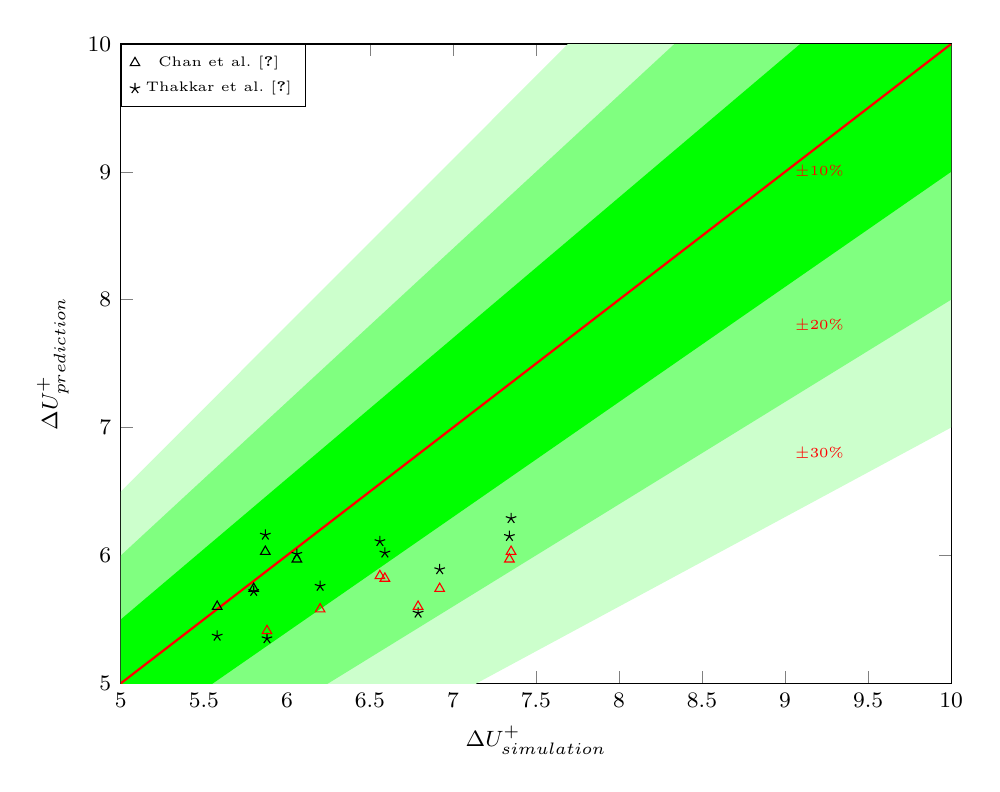
\begin{tikzpicture}[]
        \centering
        \begin{axis}[
            ylabel={$\Delta U_{prediction}^+$},
            xlabel={$\Delta U_{simulation}^+$},
            ymin=5, ymax=10,
			xmax=10,
			xmin=5,
			%xtick={-2,-1.5,...,-0.4},
            width=\linewidth,
            height=.8\linewidth,
            label style={font=\footnotesize},
			legend style={font=\tiny,at={(0,1)},anchor=north west},
            tick label style={font=\footnotesize}
            ]
            \fill[color=green!20,opacity=20] (0,0) -- (10,13) -- (10,7) -- cycle;
            \fill[color=green!50,opacity=50] (0,0) -- (10,12) -- (10,8) -- cycle;
            \fill[color=green!100,opacity=100] (0,0) -- (10,11) -- (10,9) -- cycle;
			\addplot [
            black,only marks,mark=triangle,
            ]
            coordinates{
            (5.87,6.03)
            (6.06,5.97)
            (5.80,5.74)
            (5.58,5.60)
            };
			\addlegendentry{Chan et al.~\cite{chan_macdonald_chung_hutchins_ooi_2015}}
						\addplot [
            black,only marks,mark=star,
            ]
            coordinates{
            (7.35,6.29)
            (7.34,6.15)
            (6.92,5.89)
            (6.79,5.55)
            (6.56,6.11)
            (6.59,6.02)
            (6.20,5.76)
            (5.88,5.35)
            (5.87,6.16)
            (6.06,6.01)
            (5.80,5.72)
            (5.58,5.37)
            };
			\addlegendentry{Thakkar et al.~\cite{Thakkar2017}}
						\addplot [
            red,only marks,mark=triangle,
            ]
            coordinates{
            (6.56, 5.84)
            (6.59, 5.82)
            (6.20,5.58)
            (5.88,5.41)
            (7.35,6.03)
            (7.34,5.97)
            (6.92,5.74)
            (6.79,5.60)
            };
			\addplot [
            red,thick,solid,mark=square,
            ]
            coordinates{
            (0, 0)
            (11, 11)
            };
			\node[red,right] at (axis cs: 9,9) {\tiny $\pm10\%$};
						\node[red,right] at (axis cs: 9,7.8) {\tiny $\pm20\%$};
									\node[red,right] at (axis cs: 9,6.8) {\tiny $\pm30\%$};
        \end{axis}
        \end{tikzpicture}
    \caption{$\Delta U^+$}
    \end{subfigure}\hfill
    \begin{subfigure}[t]{0.49\linewidth}
            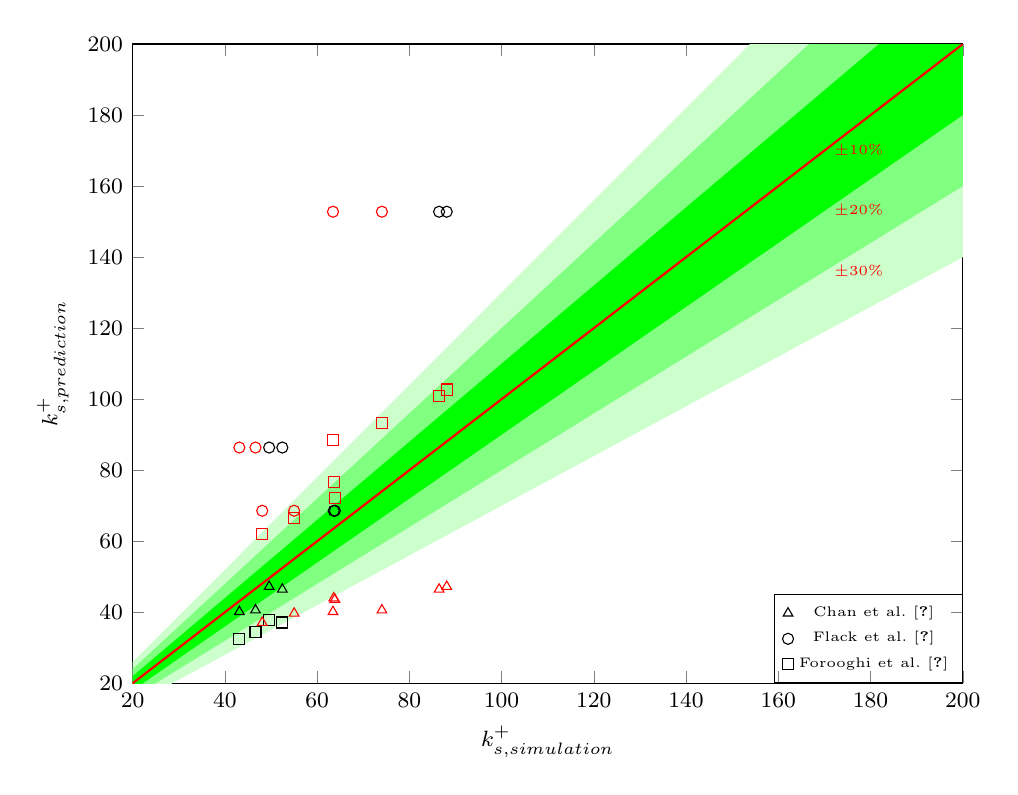
\begin{tikzpicture}[]
        \centering
        \begin{axis}[
            ylabel={$k_{s,prediction}^+$},
            xlabel={$k_{s,simulation}^+$},
            ymin=20, ymax=200,
			xmax=200,
			xmin=20,
			%xtick={-2,-1.5,...,-0.4},
            width=\linewidth,
            height=.8\linewidth,
            label style={font=\footnotesize},
			legend style={font=\tiny,at={(1,0)},anchor=south east,fill=none},
            tick label style={font=\footnotesize}
            ]
			 \fill[color=green!20,opacity=20] (0,0) -- (200,260) -- (200,140) -- cycle;
			 \fill[color=green!50,opacity=50] (0,0) -- (200,240) -- (200,160) -- cycle;
			 \fill[color=green!100,opacity=100] (0,0) -- (200,220) -- (200,180) -- cycle;

			\addplot [
            black,only marks,mark=triangle,
            ]
            coordinates{
                        (49.60,47.24)
            (52.46,46.47)
            (46.64,40.60)
            (43.14,40.14)
            };
			\addlegendentry{Chan et al.~\cite{chan_macdonald_chung_hutchins_ooi_2015}}
			\addplot [
            black,only marks,mark=o,
            ]
            coordinates{
            (63.60, 68.58)
            (63.85, 68.58)
            (88.10,152.78)
            (86.45,152.78)
            (49.60,86.38)
            (52.46,86.38)
            };
			\addlegendentry{Flack et al.~\cite{Flack2020}}
			\addplot [
            black,only marks,mark=square,
            ]
            coordinates{
            (49.60,37.78)
            (52.46,37.12)
            (46.64,34.36)
            (43.14,32.56)
            };
			\addlegendentry{Forooghi et al.~\cite{10.1115/1.4037280}}
			\addplot [
            red,only marks,mark=o,
            ]
            coordinates{
            (55.02,68.58)
            (48.10,68.58)
            (74.05,152.78)
            (63.44,152.78)
            (46.64,86.38)
            (43.14,86.38)
            };
			\addplot [
            red,only marks,mark=square,
            ]
            coordinates{
            (63.60, 76.62)
            (63.85, 72.16)
            (55.02,66.55)
            (48.10,62.12)
            (88.10,102.71)
            (86.45,100.92)
            (74.05,93.39)
            (63.44,88.52)
            };
			\addplot [
            red,only marks,mark=triangle,
            ]
            coordinates{
            (63.60, 43.98)
            (63.85, 43.61)
            (55.02,39.70)
            (48.10,37.10)
            (88.10,47.24)
            (86.45,46.47)
            (74.05,40.60)
            (63.44,40.14)

            };
						\addplot [
            red,thick,solid,mark=square,
            ]
            coordinates{
            (0, 0)
            (201, 201)
            };
			\node[red,right] at (axis cs: 170,170) {\tiny $\pm10\%$};
						\node[red,right] at (axis cs: 170,153) {\tiny $\pm20\%$};
									\node[red,right] at (axis cs: 170,136) {\tiny $\pm30\%$};
        \end{axis}
        \end{tikzpicture}
    \vspace{-0.5cm}
    \caption{$k_s^+$}
    \end{subfigure}
    \caption{Prediction vs. simulation. 10\%, 20\% and 30\% error interval are represented by green shadow. Data points within the range of fitting data are marked in red}
    \label{Corks}
\end{figure}







\section{New correlation}
\label{ML}
Basing on the research from previous sections, the crucial importance of both HPD and PS are exhibited.
A correlation model for roughness function is built with both HPD information and PS information involved.
The preliminary predictive model only serves for a deeper understanding of how roughness parameters can affect near-wall flow behaviour.\newline
Taking the advantage of the highly structured database built in present work, 4 parameters can be taken as the roughness statistical features i.e. $Sk$, $p$, $\lambda_0$ and $ES$.
Basing on the assumption that the distribution of $\Delta U^+$ obeys Gaussian distribution, a Gaussian Process Regression (GPR) model can be built.
GPR is a non-parametric regression model, in which uncertainty level of data points can be prescribed.
Rewinding the random process of roughness generation, confidence interval of the results detected from section~\cref{Rando} is applied to define the uncertainty level for the model.\newline	
Five independently generated roughness are used to assess the model.
Roughness parameters are shown in table~\ref{5more}. 
In addition to single-peak HPDs, a multi-peak Bimodal HPD is also evaluated which is labeled as $B$ in the first character.
Overview of the roughness structures are shown in Fig.~\ref{bimodal}(a-e).
The visualization of two newly included types of HPD are shown in Fig.~\ref{bimodal}(f). \newline
3-D representation of the model at $\lambda_0=0.4H$ is shown in Fig.~\ref{GPRpredict} against $Sk$ and $p$.
Confidence margins for its prediction is also provided and shown in figure with transparent planes.
As can be observed in Fig.~\ref{GPRpredict}(a), uncertainty rises at the region where no data point is present (Recall that the data set locates in $-0.48\leq Sk\leq0.48$, $-2 \leq p \leq-1$).
Testing data from table \ref{5more} are represented by circle in~\ref{GPRpredict}(a).
The corresponding roughness features are shwon with plus symbols on the bottom plane.
Red area illustrates the range of roughness parameters from training data.
The testing data within the training data range is marked in red.
In Fig.~\ref{GPRpredict}(b) predictions of $\Delta U^+$ is plotted against simulations to evaluate the model.
Prediction error are lower than $\pm 3\%$.
It is also worth to mention, that by excluding ES in the correlation model, no significant influence is observed.
Therefore, basing on the present research, it is suggested that both HPD and PS information of roughness should be included to develope a hydrodynamic correlation.
\begin{table}[h!]
        \centering
        \caption{Testing rough surfaces}
        \label{5more}
        \begin{tabular}{|c|c|c|c|c|c|c|c|}
            \hline
            Case & $\textit{Sk}$ & $p$ & $\lambda_0$($H$) & $\lambda_1$($H$)&$\Delta U^+_{simulation}$&$\Delta U^+_{prediction}$\\
            \hline
            \hline
            \textit{G754} & 0 & -0.75 & 0.4 &0.04&6.80&6.85 \\
            \textit{G154}& 0 & -1.5 & 0.4 & 0.04&6.65&6.50 \\
            \textit{P76154}& 0.76 & -1.5 & 0.4 & 0.04&7.36&7.43\\
            \textit{P7624} & 0.76 & -2 & 0.4 & 0.04&7.35&7.17 \\
            \textit{BN58154}& -0.58 & -1.5 & 0.4& 0.04&6.05&5.93\\
            \hline
            \end{tabular}
            \end{table}
                        \begin{figure}[H]
                \centering
                                \begin{subfigure}[t]{0.5\linewidth}
                \input{tikz/G0754}
                \caption{Roughness map G754}
                \end{subfigure}\hfill%
                \begin{subfigure}[t]{0.5\linewidth}
                \input{tikz/G154}
                \caption{Roughness map G154}
                \end{subfigure}\hfill%
                \begin{subfigure}[t]{0.5\linewidth}
                \input{tikz/P76154}
                \caption{Roughness map P76154}
                \end{subfigure}\hfill%
                \begin{subfigure}[t]{0.5\linewidth}
                \begin{tikzpicture}
\begin{axis}[
		xlabel=$L_x$,
		ylabel=$L_z$,
		xmin=0,xmax=2.0,
		ymin=0,ymax=0.4,
		y dir=reverse,
		clip=true,
		set layers,
		clip mode=individual,
		height=0.38\linewidth,
		width=.83\linewidth,
		xtick={0,0.4,...,2.0},
		ytick={0,0.2,...,0.4},
		label style={font=\footnotesize},
		tick label style={font=\footnotesize},
		colorbar,
		point meta min=0.0,
		point meta max=0.1227,
		colorbar style={
		ytick={0,0.12},
		width=0.2cm
		}
	]
	\centering
\addplot [thick, color=blue, on layer=axis background]
graphics[xmin=0,ymin=0,xmax=2.0,ymax=0.4]{Figures/P7624.png};

\end{axis}
\end{tikzpicture}
                \caption{Roughness map P7624}
                \end{subfigure}\hfill%
                \begin{subfigure}[t]{0.5\linewidth}
                \input{tikz/bimodalsurface}
                \caption{Roughness map BN58154}
                \end{subfigure}\hfill%
                \begin{subfigure}[t]{0.44\linewidth}
                        \begin{tikzpicture}[]
        \centering
        \begin{axis}[
            ylabel={Posibility density},
            xlabel={Height},
            ymin=0, ymax=0.05,
			%xmin=1,xmax=500,
            width=1\textwidth,
            height=1\textwidth,
			%xmode=log,
            %legend style={font=\tiny,at={(axis cs:9,-1)},anchor=south west},
            legend style={font=\tiny,at={(0,1)},anchor=north west,fill=none},
            label style={font=\footnotesize},
            tick label style={font=\footnotesize}
            ]
            \addplot [
            black,solid,thick,
            ]
            table [x=X, y=Y,col sep=comma]{CSV/BimodalPDF1.csv};
            \addlegendentry{Double-peak $Sk=-0.58$}
            \addplot [
            black,dashed,thick,
            ]
            table [x=X, y=Y,col sep=comma]{CSV/P76PDF1.csv};
            \addlegendentry{Single-peak $Sk=0.76$}
        \end{axis}
        \end{tikzpicture}
                \caption{Two new types of HPD applied in testing set (\full: double-peak HPD $Sk=-0.58$, \dashed: single-peak HPD $Sk=0.76$}
                \end{subfigure}
                \caption{Rough surfaces \& additional tested HPDs }
                \label{bimodal}
            \end{figure} 
\begin{figure}
    \centering
    \begin{subfigure}[c]{0.8\linewidth}
    \centering
    \includegraphics[width=\linewidth]{Figures/GPRpredict.png}
    %\begin{tikzpicture}
\begin{axis}[view={30}{20},
		xlabel=$Sk$,
		ylabel=$p$,
		zlabel=$\Delta U^+$,
		zmin=5,
		%colormap/parula,
		mesh/cols=100,
		height=.8\linewidth,
		width=1\linewidth,
		%colorbar,
		]
					\addplot3 [
            black,only marks,mark=+,
            ]
            coordinates{
            (0,-0.75,5)
            (0.76,-1.5,5)
            (0.76,-2,5)
            (-0.58,-1.5,5)
            };
            					\addplot3 [
            red,only marks,mark=+,
            ]
            coordinates{
            (0,-1.5,5)
            };
		\fill[color=red!60,opacity=100] (-0.48,-2,5) -- (-0.48,-1,5) -- (0.48,-1,5) -- (0.48,-2,5) -- cycle;
		  \addplot3 [surf,shader=interp,opacity=0.4]
  table[x=Sk, y=PSslope, z=Down, col sep=comma] {CSV/GPRpredict.csv};
  \addplot3 [
            black!30,dashed,no marks
            ]
            coordinates{
            (0,-0.75,5)
            (0,-0.75,6.80)
            };
              \addplot3 [
            red!30,dashed,no marks
            ]
            coordinates{
            (0,-1.5,5)
            (0,-1.5,6.65)
            };
              \addplot3 [
            black!30,dashed,no marks
            ]
            coordinates{
            (0.76,-1.5,5)
            (0.76,-1.5,7.36)
            };
                          \addplot3 [
            black!30,dashed,no marks
            ]
            coordinates{
            (0.76,-2,5)
            (0.76,-2,7.35)
            };
                          \addplot3 [
            black!30,dashed,no marks
            ]
            coordinates{
            (-0.58,-1.5,5)
            (-0.58,-1.5,6.05)
            };
\addplot3 [surf,shader=interp,color=blue]
  table[x=Sk, y=PSslope, z=Y, col sep=comma] {CSV/GPRpredict.csv};
    \addplot3 [surf,shader=interp,opacity=0.4]
  table[x=Sk, y=PSslope, z=UP, col sep=comma] {CSV/GPRpredict.csv};
			\addplot3 [
            black,only marks,mark=o,
            ]
            coordinates{
            (0,-0.75,6.80)
            (0.76,-1.5,7.36)
            (0.76,-2,7.35)
            (-0.58,-1.5,6.05)
            };
            			\addplot3 [
                        red,only marks,mark=o,
            ]
            coordinates{
            (0,-1.5,6.65)
            };

\end{axis}
\end{tikzpicture}
        \caption{Prediction by GPR model, $\medcircle$ represent testing roughness, corresponding roughness parameters are localized by $+$, transparent planes are 95\% confidence bound, the range of training roughness parameters are illustrated by red plane, testing data within the training data range is marked in red.}
    \end{subfigure}\hfill%
    \begin{subfigure}[c]{0.8\linewidth}
    \centering

            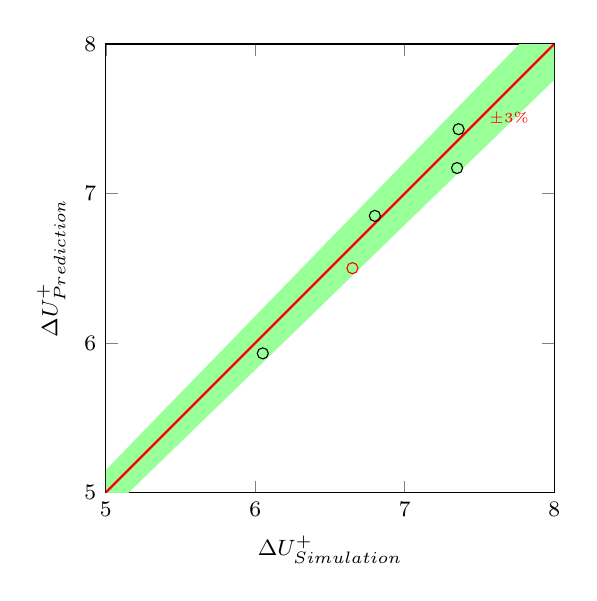
\begin{tikzpicture}[]
        \centering
        \begin{axis}[
            ylabel={$\Delta U_{Prediction}^+$},
            xlabel={$\Delta U_{Simulation}^+$},
            ymin=5, ymax=8,
			xmax=8,
			xmin=5,
			%xtick={-2,-1.5,...,-0.4},
            width=.6\textwidth,
            height=.6\textwidth,
            label style={font=\footnotesize},
			legend style={font=\tiny,at={(0,1)},anchor=north west},
            tick label style={font=\footnotesize}
            ]
			\addplot [
            black,only marks,mark=o,mark size=2pt
            ]
            coordinates{
            (6.80, 6.85)
			(7.36,7.43)
			(7.35,7.17)
			(6.05,5.93)
            };
            			\addplot [
                        red,only marks,mark=o,mark size=2pt
            ]
            coordinates{
            (6.65,6.50)
            };
			 \fill[color=green!40,opacity=40] (0,0) -- (9,9.27) -- (9,8.73) -- cycle;
						\addplot [
            red,thick,solid,mark=square,
            ]
            coordinates{
            (0, 0)
            (9, 9)
            };
			\node[red,right] at (axis cs: 7.5,7.5) {\tiny $\pm3\%$};
        \end{axis}
        \end{tikzpicture}
    \caption{$\Delta U^+$ predictions against simulations, Green shadow indicates prediction error interval of $\pm3\%$ around $\Delta U_{Simulation}^+=\Delta U_{Prediction}^+$ (\Rfull). Testing data within the training data range is marked in red}
    \end{subfigure}
    \caption{GPR predictions}
    \label{GPRpredict}
\end{figure}
\newpage
\section{Conclusion}
DNS of irregular roughness in minimal channel is evaluated in present work. 
A number of irregular roughness of different types are simulated in minimal channels at $Re_\tau\approx500$.
Prediction error by minimal channels relative to full span channel are lower than $\pm5\%$. 
The possibility of studying equivalent roughness height $k_s$ in minimal channel is also demonstrated by simulating irregular roughness $G24$ in minimal channel at $Re_\tau=250-1000$. 
The mathematical random roughness generation algorithm by Pérez-Ràfols~\cite{PEREZRAFOLS2019591} gives researchers possibility of parametrically varying roughness parameters of interest, which enables the systematic study of irregular roughness. 
Three roughness parameters are taken into study, namely $Sk$, $p$ and $\lambda_0$. 
Effect of the roughness parameters are found identical with previous research that skin friction increases with $Sk$. 
Whats more, by adjusting roughness PS, it is also shown that there is a certain range of roughness wavelength that is dominant to skin friction.
Three existing roughness correlations are examined in present work.
The difficulty of developing a general predictive tool is shown.
It is implied by comparing the models by Chan et al.~\cite{chan_macdonald_chung_hutchins_ooi_2015}, Thakkar et al.~\cite{Thakkar2017}, Flack et al.\cite{Flack2020} and Forooghi et al.~\cite{10.1115/1.4037280} that more roughness parameters should be included into the correlation. 
The model by Forooghi et al. gives the best prediction with error $\leq\pm30\%$ which involves both $Sk$ and ES in the correlation. 
This indicates that both height distribution information as well as the spatial distribution information of the roughness should be involved in developing a correlation model. 
\newpage
\printbibliography
\end{document}
